\documentclass{article}
\usepackage[utf8]{inputenc}
\usepackage[parfill]{parskip}
\usepackage{graphicx}
\usepackage{listings}
\usepackage[usenames,dvipsnames]{color}
\usepackage{etex}
\reserveinserts{18}
\usepackage{morefloats}
\usepackage[margin=1in]{geometry}

\title{CS909: Week 10}
\author{1037559}
\date{}

\begin{document}

\maketitle

\section{Introduction}
This report details the implementation of the text classification system required for the week 10 assignment. It describes in detail each stage of the assignment, the reasons for any decisions made and the outcomes of these. The first section corresponds to reading in the data, and then feature selection and reduction is discussed. The classification task is then described and evaluated, followed by the clustering task. Finally conclusions are made. Any results can be found in the appendices following the report. The code for the implementation may be found on GitHub\footnote{https://github.com/RuthRainbow/DataMining}. The assignment was implemented using Python.

\section{Data Input}
The first task was to read in the data, which is in SGM format. This was done using the \verb|BeautifulSoup| module for Python. This module is able to parse SGM files so data can be extracted by tag, which is useful for this assignment as it allows items such as the topic can easily be extracted. For each data file a \verb|BeautifulSoup| object was created, and these added to a list of `soups'.

The next task was to extract the relevant tags from the soups. \verb|BeautifulSoup| objects provide methods for extracting tags easily, for example using the methods \verb|find_all| and \verb|findChildren|. \verb|find_all| was used to find all text tags and reuters tags. Within the reuters tags the lewissplit and topic attributes were extracted. Topics were extracted in this way in order to provide a list of topics where an article includes multiple topics.

All extracted entries are then examined. Firstly the body is either loaded in already preprocessed or preprocessing takes place, as discussed in the preprocessing section. This is to avoid repeating preprocessing, which is computationally expensive. Preprocessing is only carried out once per body, to avoid repetition with multiple topics. The corresponding topics are then checked to see if they are a topic we are interested in. If so the lewis attribute is checked to find whether to place the text in the training or test lists. The text is added one time for every topic tag it contains that we are interested in. This is so it can be labelled with every relevant label, as each text in the classification may only have one label. All texts are also added once to a separate list in order to be used by the classification algorithms, which look at all data.

The table below shows the frequency of the main topic labels for classification obtained over the 22 SGM files:
\\
\begin{center}
\begin{tabular}{l | l}
Topic & Frequency \\ \hline
earn & 3961 \\
acq & 2367 \\
money-fx & 717 \\
grain & 583 \\
crude & 580 \\
trade & 487 \\
interest & 480 \\
ship & 287 \\
wheat & 283 \\
corn & 239 \\ \hline
Total number of texts: 9984 \\
\end{tabular}
\end{center}

Taking all topics into account 120 topics were present.

\section{Preprocessing}
After the relevant texts had been extracted preprocessing takes place. This is done text by text when extracting text tags as described above using the \verb|preprocess| function, and is implemented in the \verb|preprocessing.py| file.

For the basic preprocessing firstly the text is changed to utf-8 encoding so all characters can be manipulated by the Python string methods. Secondly the title and date are removed, as these should not be part of the text. Next the word ``Reuter'' is removed from the end of the text - this is present as it is part of the tag for all texts. The text is then converted to lower case and punctuation and numbers removed, using the \verb|regex| module for Python. An example of the effects of this preprocessing can be seen below:

Before preprocessing (raw data):

``U.K. MONEY MARKET SHORTAGE FORECAST REVISED DOWN
    LONDON, March 3 - The Bank of England said it had revised
its forecast of the shortage in the money market down to 450
mln stg before taking account of its morning operations. At
noon the bank had estimated the shortfall at 500 mln stg.
 REUTER
''

Post basic preprocessing:

``the bank of england said it had revised its forecast of the shortage in the money market down to mln stg before taking account of its morning operations at noon the bank had estimated the shortfall at mln stg''

Further preprocessing is also carried out. Firstly Stopwords are removed, using an English corpora as all stopwords should be English. This corpora of stopwords was obtained through the \verb|nltk| module. Next a spell corrector from the \verb|WordNet| module is used and a part of speech tagger applied. After this words are lemmatised in order to obtain the ``stem'' of a word, for example ``runner'' should be reduced to ``run''. This requires the tags to be in a slightly simpler form, so a helper method was included to convert to this form. An English language lemmatiser is then used from the \verb|nltk| module. Optionally a named entity tagger may also be applied to replace things such as company names in the texts. This is optional as it is very computationally expensive and may take a long time. The results of this can be seen in the example below, where it's clear that words have been lemmatised fairly successfully:

``[u'bank', u'england', 'say', u'revise', u'forecast', u'shortage', u'money', u'market', u'man', u'st', u'take', u'account', u'morning', u'operation', u'noon', u'bank', u'estimate', u'shortfall', u'man', u'st']''

\section{Feature Selection}
A number of different feature selection mechanisms were implemented and evaluated to determine the method must suitable for the task. Features are selected based on the words present or absent in each text.

\subsection{Bag of words}
Firstly, a `bag of words' approach was implemented, where each text is represented as a vector where every column represents a word in the vocabulary. Entries in the vector indicate the presence or absence of a word. This creates a sparse vector representation of every text.

This approach was implemented in two ways. Firstly, using \verb|nltk| to create a dictionary of all vocabulary and using this to convert each text. This allowed any words which appeared in less than $n$ documents to be filtered out to attempt to reduce the dimensionality of the final vectors. The below shows the results of converting a text to a bag of words:

[(0, 2), (1, 1), (2, 1), (3, 1), (4, 1), (5, 2), (6, 1), (7, 1), (8, 1), (9, 2), (10, 2), (11, 1), (12, 1), (13, 2), (14, 1), (15, 1), (16, 1), (17, 1), (18, 1), (19, 1), (20, 1), (21, 1), (22, 5), (23, 1), (24, 1), (25, 5), (26, 2), (27, 1), (28, 2), (29, 1), (30, 1), (31, 1), (32, 2), (33, 5), (34, 4), (35, 1), (36, 2), (37, 1), (38, 3), (39, 2), (40, 6), (41, 2), (42, 1), (43, 3), (44, 1), (45, 4), (46, 2)]

The second approach used scilearn's \verb|CountVectorizer|. This simply creates feature vectors for each text with a frequency count for each ``feature'' or word in the vocabulary. Optionally this can be used as a binary vectoriser, indicating only the presence or absence of a word.

\subsection{Term Frequency - Inverse Document Frequency (TF-IDF)}
This approach attempts to normalise the data and take into account the relative frequencies of words in the text in comparison to the frequency over all texts. This approach provides more information than the previous approach as it also takes into account frequency, which may be important to classification.

The first implementation of this was provided by manually summing the frequencies of all words and applying the formaluae for term frequency (TF) and inverse document frequency (IDF) as defined in the lectures:

\begin{center}
$tf(t, d) = \frac{Frequency\:of\:term\:t\:in\:document\:d}{max.\:frequency\:of\:t\:in\:any\:doc\:d}$
\end{center}

\begin{center}
$idf(t, D) = log\frac{|D|}{df(t,D)}$
\end{center}

where $D$ is the set of all documents. The words with the highest n TF-IDF scores can then be used as features. The example below shows a text and it's associated TF-IDF features, to three decimal places:

\begin{verbatim}
The U.S. Agriculture Department reported the farmer-owned
reserve national five-day average price through February 25
as follows (Dlrs/Bu-Sorghum Cwt) -
         Natl   Loan           Release   Call
         Avge   Rate-X  Level    Price  Price
 Wheat   2.55   2.40       IV     4.65     --
                            V     4.65     --
                           VI     4.45     --
 Corn    1.35   1.92       IV     3.15   3.15
                            V     3.25     --
 X - 1986 Rates.

          Natl   Loan          Release   Call
          Avge   Rate-X  Level   Price  Price
 Oats     1.24   0.99        V    1.65    -- 
 Barley   n.a.   1.56       IV    2.55   2.55
                             V    2.65    -- 
 Sorghum  2.34   3.25-Y     IV    5.36   5.36
                             V    5.54    -- 
    Reserves I, II and III have matured. Level IV reflects
grain entered after Oct 6, 1981 for feedgrain and after July
23, 1981 for wheat. Level V wheat/barley after 5/14/82,
corn/sorghum after 7/1/82. Level VI covers wheat entered after
January 19, 1984.  X-1986 rates. Y-dlrs per CWT (100 lbs).
n.a.-not available.
\end{verbatim}

[('iv', 0.346), ('x', 0.266), ('level', 0.163), ('age', 0.148), ('vi', 0.147), ('y', 0.144), ('price', 0.122), ('sorghum', 0.107), ('rate', 0.107), ('reserve', 0.101)]

It can be seen that the Roman numeral features had very high TFIDF values. This may be because this sort of report only appears for topics related to wheat, grain and corn, as this article was labelled. Sorghum is also an important feature, as this is another cereal crop.

The second implementation used the \verb|TfidfVectorizer| from the SciLearn module. This vectoriser can also be used for some preprocessing steps, such as removing accents and stop words, however when the data is already preprocessed this is not necessary. This vectoriser also normalises the features, as TFIDF does this automatically.

\subsection{Feature Reduction}
Feature reduction is lastly applied to all feature selection methods in order to eliminate irrelevant or rare features from the dataset and reduce the dimensionality of the vectors to further focus on more relevant features.

From the SciLearn module a $\chi^2$ test was applied to select the k best features. This test determines how relevant words are to determining a class, and the $k$ most relevant features are retained for each class. However it was found that this was detrimental to results and reduced the accuracies obtained, so this was left commented out for collecting results. This reduced accuracy suggests a greater number of features were required; however there was not enough memory to run a $\chi^2$ test to select enough features to cause an improvement in accuracy with this implementation.

\subsubsection{Clustering}
It was found that some clustering methods required dense vectors, rather than the sparse vectors produced by the feature selection methods. There is also a greater number of examples for these algorithms to fit as the algorithms are unsupervised so the data is not split into testing and training sets, and we do not only select the most popular topics.

To further reduce dimensionality and convert to dense vectors a form of Principle Components Analysis (PCA) is applied. The implementation of this was carried out using \verb|TruncatedSVD| from SciLearn, which is a variant of PCA that is able to work on feature vectors in a memory efficient way. This was required as the implementation of PCA was not able to keep all texts in memory with the full data set. After this the vectors need to be renormalised for the clustering algorithms. 

\subsection{Topic Models}
Topic models were created using the \verb|gensim| module. A `bag of words' approach was used as described above. All texts are converted to vectors, mapping word identifiers to the frequency of the words occurring in that text. These vectors can then be used to create topic models, which give probability distributions for each text appearing in a given number of topics. The models were created using 10 topics, as we know this is the number present from the preprocessing.

A Latent Dirichlet Allocation (LDA) model was created, as described in the lectures. This was created by passing the dictionary and the word feature vectors into an \verb|LdaModel| object (from the \verb|gensim| module).

The below shows the ten most important features for each of the ten topics:

\begin{enumerate}
\item 0.186*v + 0.134*man + 0.069*net + 0.055*day + 0.053*loss + 0.032*rev + 0.030*profit + 0.020*note + 0.016*ave + 0.015*sale
\item 0.035*april + 0.032*record + 0.027*pay + 0.026*v + 0.024*prior + 0.018*only + 0.012*rate + 0.012*dollar + 0.007*payable + 0.007*june
\item 0.031*share + 0.019*day + 0.018*offer + 0.013*stock + 0.012*company + 0.011*man + 0.011*put + 0.009*common + 0.008*tender + 0.008*shareholder
\item 0.019*trade + 0.012*japan + 0.009*market + 0.007*country + 0.006*state + 0.006*price + 0.006*policy + 0.006*c + 0.006*japanese + 0.006*import
\item 0.017*put + 0.015*day + 0.012*man + 0.010*company + 0.009*new + 0.008*corp + 0.007*year + 0.007*bank + 0.006*sale + 0.005*acquire
\item 0.047*day + 0.024*man + 0.014*year + 0.013*share + 0.012*company + 0.012*quarter + 0.010*put + 0.010*first + 0.009*expect + 0.008*oil
\item 0.030*rate + 0.026*bank + 0.024*put + 0.020*market + 0.010*man + 0.009*money + 0.008*central + 0.008*reserve + 0.008*day + 0.007*st
\item 0.023*share + 0.015*company + 0.013*put + 0.010*stock + 0.009*security + 0.008*stake + 0.008*exchange + 0.007*corp + 0.007*common + 0.007*co
\item 0.024*oil + 0.012*gulf + 0.006*put + 0.006*attack + 0.006*state + 0.006*italian + 0.005*ship + 0.005*banker + 0.004*platform + 0.004*gas
\item 0.048*man + 0.033*tone + 0.019*year + 0.016*put + 0.016*export + 0.015*wheat + 0.012*last + 0.010*day + 0.009*grain + 0.007*import
\end{enumerate}

From these features we can see try to guess the corresponding topics. For example topic 10 seems to be related to either wheat or grain, as both of these key words have been picked out. This also suggests a large overlap in these two topics. For topic 1 `v' has been picked out. This is the lemmatised form of `vs', which is used in `earn' topics very frequently. Topic 9 seems to refer to `crude' as it contains a lot of words to do with oil. From this data it also seems important not to filter out dates - topic 2 has `april' as its most important feature, as it may refer to a topic which often creates reports in this month. These words represent possible features for each topic.

Here are the results obtained from the first six texts, to three decimal places:

[(0, 0.140), (6, 0.851)]

[(0, 0.193), (5, 0.023), (6, 0.423), (9, 0.355)]

[(2, 0.969)]

[(2, 0.864), (4, 0.109), (8, 0.021)]

[(0, 0.927), (6, 0.044)]

[(2, 0.305), (5, 0.683)]

It can be seen that a variety of probability distributions are obtained, denoting which topic each text is most likely to be in. For example, the topic model seems fairly sure that the 5th example comes from topic 0, which corresponds to `earn' from the intuition above.

\section{Classifier Design \& Implementation}
Classification was carried out using the features selected with a variety of different classifiers. For each a number of metrics were collected in order to effectively compare the methods. A variety of different classifiers were applied in order to compare their effectiveness at classifying the texts into topics. Training and test data sets were obtained using the lewissplit tag as described in the data input section.

\subsection{TextBlob module}
The \verb|TextBlob| module contains some simple classifier implementations which were experimented with first. These classifiers use their own feature selection method which creates topic probabilities based on the presence or absence of words or characters. Two classifier implementations were used; firstly a na{\"i}ve Bayes classifier and secondly a decision tree classifier. However not a lot of metrics are easily available for these classes so only accuracy was compared. These classifiers are interesting as they allow you to view the most important features they used for each class, however due to the lack of metrics the main classification was done using the SciLearn model, as described below. This code was separated out and can be found in the file \verb|txtblob.py|.

\subsection{SciLearn module}
The SciLearn module provides a much greater variety of classifiers which are more customisable with a large number of optional flags. The output of these is also much more easily obtainable, with methods to provide metrics for the classifier and for each class. The code using SciLearn can be found in the file \verb|scilearn.py|.

To make the code more readable a \verb|classify| method was written which takes in a classifier class as a parameter. This fits the classifier to the training data and uses this to predict labels for the test data. It then prints the metrics as discussed below.

Each classifier is trained using 10-fold cross validation, obtaining splits from the \verb|KFold| class. This aims to obtain independent estimates of how well the classifier will perform on unseen data. The method shuffles the data and returns the indexes from which each fold should be taken. Each classifier is trained and tested on all folds and the accuracy metrics for each fold recorded. From the 10 folds the mean and standard deviation of the accuracy is calculated using \verb|numpy|. These are used to calculate 95\% confidence intervals for the accuracy. It is assumed, by the central limit theorem, that the accuracy of each classifier follows a Normal distribution, since there are enough training examples for the distribution not to be skewed. Confidence intervals are then printed after all 10 folds have been completed. The classifier which obtained the highest mean accuracy is then trained over the entire training set, and the statistics of this output via the \verb|classify| method.

The classifiers used can be split into four different categories, and will be discussed in the subsections below.

\subsubsection{Na{\"i}ve Bayes}
Na{\"i}ve Bayes methods are often used for text classification tasks as a baseline. In this case three different methods were used and the results compared, as discussed in the evaluation section. Each will be described in turn, as well as any parameters chosen.

\verb|GaussianNB| (Gaussian Na{\"i}ve Bayes) assumes each class follows a Gaussian distribution. This is usually useful for continuous data, so it is expected that the TF-IDF vectorisation will be more relevant here.

\verb|MultinomialNB| (Multinomial Na{\"i}ve Bayes) uses a multinomial event model. This is expected to be relevant here in a multiclass scenario so should perform well. The default Laplascian parameter is used for smoothing and class prior probabilities are learnt. This is important here as there are likely to be many texts which contain a count of 0 for many features. This should be used for discrete data, so should perform better for the count vectoriser.

\verb|BernoulliNB| (Bernoulli Na{\"i}ve Bayes) uses a Bernoulli event model assuming a binary vectorisation. Because of this a parameter is applied as a threshold of how to convert the vector into binary - 1 is given, so this is expected to perform poorly for TFIDF. The same smoothing is used and again class prior probabilities are learnt. This model is simpler than Multinomial and so may overfit less.

\subsubsection{Tree based}
Decision tree methods for classification can work well, however they have a high tendency to overfit. As this task uses sparse vectors of features it is likely that overfitting will be reduced as there should be a number of examples from each class with diverse features.

\verb|DecisionTreeClassifier| implements a decision tree classifier. Information gain is used for deciding whether to split attributes, as described in the lectures. The minimum samples per split and leaf were changed to 5 (greater than the default), as the amount of data is large and we want to avoid overfitting.

\verb|RandomForestClassifier| is an ensemble method using decision trees. The same parameters are used as for the decision tree classifier in order to be able to compare the two.

\subsubsection{Linear}
Linear classification methods create decision boundaries to separate the data into classes in an N-dimensional space, where N is the number of features. These methods tend to underfit, so should be less effected by overlapping topics.

\verb|Perceptron| implements a linear perceptron, and also centralises the data. This is not expected to perform well as the data is not expected to be linearly separable into classes. However; perceptrons are often used for text classification tasks and have been shown to perform well in the past.

\verb|LinearSVC| was used as a scalable implementation of a Support Vector Machine (SVM) with a linear kernel. This kernel was used as the default, and because studies have shown that the performance depends more on the parameters than the type of kernel. Linear SVMs also require an error term parameter C. The algorithm was run over a range of values in order to find the best value for this, and it was found 0.7 gave the best results, although by a very small margin. The data is again centralised using a flag. SVMs have often been shown to work well for classification tasks so this classifier should do well.

\subsubsection{Nearest neighbours}
\verb|KNeighborsClassifier| attempts to predict a class using an example's nearest neighbours and euclidean distance. The number of neighbours to check was increased to 10 in order to avoid classification based on outliers. 

\verb|NearestCentroid| represents classes via a representative or centroid.  The nearest centroid is used to classify an example.

\subsection{Metrics}
A number of different metrics will be used to evaluate the clustering algorithms. Most of these are available only for the SciLearn classifier algorithms, which will form the focus of most of the evaluation. All metrics take into account the multi-class scenario, using multi-class true and false positives and negatives (TP, FP, TN, FN).

The first of these, as used by both TextBlob and SciLearn, is the accuracy of the classifier. This metric describes where the label was predicted correctly for examples (TPs), and is normalised to a value between 0 and 1, where 1 is all examples being classified correctly. This metric will be used as described above during 10-fold cross validation to discover confidence intervals for the accuracy of each of the SciLearn classifiers.

The second metric to be used is the recall for each class over each of the 10 folds. This represents the formula $\frac{TP}{TP+FN}$, which informs about the classifier's ability to label positive examples correctly. Precision will also be reported for each class, which uses the formula $\frac{TP}{TP+FP}$ and represents a classifier's ability to label negative examples correctly. The f1 score represents the harmonic mean between precision and recall, giving an average value. 

The micro and macro averages for both precision and recall will also be reported, over all classes. The macro average averages the precision and recall values for each class, whereas the micro average calculates precision and recall using the average TP, FP and FN values for each class.

\section{Classifier Evaluation}
Each of the classifiers described above was trained over the training set, manipulated as described in the feature selection section, and then tested for the metrics described above over the test set. The results of this will be described in this section of the report.

\subsection{TextBlob classification}
Firstly the performance of the TextBlob classifiers will be described. For these there were not a lot of metrics easily available so only accuracy is displayed. These classifiers are interesting as they allow you to view the most informative features. These classifiers are also significantly slower than the SciLearn equivalents.

The na{\"i}ve Bayes classifier obtained an accuracy over the test set of 72.8\%. Table 1 displays the most informative features the classifier found when comparing classes. For example, the first rule states that if a text contains the word `wheat', it's 987 times more likely to be in the `wheat' topic rather than the `acq' topic. There are many features with a large likelihood, suggesting some features are very informative. However this shows that no rules were found separating the most alike topics: `wheat', `corn' and `grain'. There is only one rule listed here for `grain', suggesting that the training texts do not have any particularly distinguishing features here. This is probably due to the lower number of training examples and similarity to the `grain' topic. In contrast there are a lot of rules for `earn', signifying this is a much more distinctive topic.

The decision tree classifier performed better than the na{\"i}ve Bayes classifier, obtaining an accuracy of 78.2\%. However this took a lot longer to run - this may be because a very large number of features were selected and the splitting metric had to be calculated for each.

\begin{table}
\begin{tabular}{l|l|l}
\textbf{Rule} & \textbf{Topics} & \textbf{Likelihood}\\ \hline
	contains(wheat) = True &            wheat : acq &   987.0 : 1.0\\
   contains(agriculture) = True &            wheat : earn   & 964.9 : 1.0\\
        contains(farmer) = True   &           corn : earn   &    399.9 : 1.0\\
         contains(grain) = True     &         corn : earn   &    358.3 : 1.0\\
      contains(minister) = True       &      trade : earn   & 324.3 : 1.0\\
      contains(monetary) = True         &   money-fx : earn   &    317.9 : 1.0\\
   contains(enhancement) = True           &  wheat : earn   &    300.7 : 1.0\\
 contains(protectionist) = True             & trade : earn   & 292.2 : 1.0\\
      contains(shortage) = True &           money-fx : earn   &    285.9 : 1.0\\
         contains(maize) = True   &           corn : acq    & 283.3 : 1.0\\
          contains(port) = True     &         ship : earn   &    277.9 : 1.0\\
          contains(feed) = True       &     interest : earn   &    266.7 : 1.0\\
          contains(tone) = True         &    wheat : acq    &    259.5 : 1.0\\
           contains(rev) = True           &   earn : acq    &    228.4 : 1.0\\
     contains(economist) = True &           interest : earn   &    222.7 : 1.0\\
    contains(assistance) = True   &         money-fx : earn   & 211.3 : 1.0\\
         contains(cargo) = True     &         ship : earn   &    204.6 : 1.0\\
             contains(v) = True       &       earn : acq    & 200.2 : 1.0\\
       contains(loading) = True         &     ship : earn   &    196.9 : 1.0\\
      contains(treasury) = True           & money-fx : earn   & 194.1 : 1.0\\
        contains(cereal) = True             & wheat : earn   &    193.0 : 1.0\\
          contains(corn) = True &             corn : earn   &    191.1 : 1.0\\
     contains(committee) = True   &          trade : earn   &    184.7 : 1.0\\
       contains(subsidy) = True     &        wheat : earn   & 184.0 : 1.0 \\
       contains(council) = True       &      trade : earn   & 178.4 : 1.0 \\
       contains(tonne) = True          &  wheat : acq    &    177.8 : 1.0\\
        contains(moscow) = True       &     wheat : earn   & 175.0 : 1.0\\
     contains(statistic) = True      &      trade : earn   & 173.3 : 1.0\\
        contains(taiwan) = True     &       trade : earn   &    173.3 : 1.0\\
  contains(intervention) = True    &       money-fx : acq    &    172.3 : 1.0\\
        contains(attack) = True   &          ship : earn   &    168.1 : 1.0\\
          contains(hour) = True  &           ship : earn & 168.1 : 1.0\\
          contains(crop) = True &           grain : acq  &    164.5 : 1.0\\
       contains(ecuador) = True &            crude : earn &    163.6 : 1.0\\
       contains(acreage) = True            & corn : earn &    161.0 : 1.0\\
        contains(escort) = True           &  ship : earn & 158.5 : 1.0\\
         contains(coast) = True          &   ship : earn &    152.7 : 1.0\\
         contains(visit) = True         &   trade : earn &    152.6 : 1.0\\
      contains(governor) = True        &   money-fx : earn & 151.0 : 1.0\\
      contains(congress) = True       &     trade : earn &    144.3 : 1.0\\
       contains(deficit) = True      &      trade : earn &    143.8 : 1.0\\
        contains(soviet) = True     &       wheat : acq  &    143.8 : 1.0\\
       contains(textile) = True    &        trade : earn &    142.2 : 1.0\\
         contains(usual) = True   &          corn : earn  & 140.2 : 1.0\\
        contains(impose) = True  &          trade : earn & 138.1 : 1.0\\
    contains(washington) = True   &         trade : earn &    137.1 : 1.0\\
   contains(cooperation) = True   &         trade : earn & 137.1 : 1.0\\
      contains(sanction) = True  &          trade : earn  &    137.1 : 1.0\\
            contains(tr) = True &            earn : acq  &    133.4 : 1.0\\
        contains(winter) = True  &          wheat : earn  & 132.7 : 1.0\\
\end{tabular}
\caption{Features discovered by the TextBlob Na{\"i}ve Bayes classifier}
\end{table}

\subsection{SciLearn classification}
For SciLearn many more metrics were easily available, such as the f1 score and macro and micro averaged precision and recall. As 10-fold cross validation was also used we can create confidence intervals for the classifier accuracy. The results for SciLearn classification can be found in the appendix.

\subsubsection{Vectorisers}
Firstly the best classifier from the three variations of vectorisation will be compared. \verb|MultinomialNB| obtained the highest mean accuracy for both the count vectoriser and the binary vectoriser, and obtained accuracies of 81.6\% and 81.1\% respectively. The best classifier for the TFIDF vectoriser was the  \verb|LinearSVC|, which obtained an accuracy of 84.2\% over the test data. This shows that a more accurate classifier was obtained when using TFIDF. The macro and micro precision and recall values were also higher for TFIDF. The results from count and binary suggest that the actual count of features rather than simply the presence doesn't have a lot of impact on the success of the na{\"i}ve Bayes classifier. SVM seemed to work better on results normalised as in TFIDF. All three vectorisers performed better than the TextBlob classifiers - this could be because of the improved algorithm implementation or improved feature selection.

For the binary vectoriser it can be noted that the best classifier was completely unsuccessful at classifying the topics with the lowest support. For both 'wheat' and 'corn' the best classifier, \verb|MultinomialNB|, obtained precision and recall of 0, with no instances being classified correctly. This suggests that the binary vectoriser requires a greater amount of support. These two categories also convey fairly similar things so it could be considered to merge these topics; grain is also likely to have a high level of overlap with these two and is consistently classified poorly so could be merged. The TFIDF vectoriser and the count vectorisers perform similarly on the topics with low support, suggesting either of these methods are appropriate when classifying with few examples.

As the TFIDF vectoriser was the most successful we will look at the results for the classifiers obtained from this method of feature selection more closely. For the best classifier, \verb|LinearSVC|, it can be seen that the performance greatly varied over topics. For example the classifier performed extremely well for the 'earn' category, with an f1-score of 97\%. This accuracy is far above that obtained by the other vectorisers and is probably why the classifier overall is the most accurate. This suggests TFIDF vectorisation is the best method for classification with large numbers of support. This could be due to the normalisation that takes place. 

Overall for TFIDF the precision and recall average values do not differ very much - this suggests the classifier is equally likely to classify false positives and false negatives. This seems to suggest there are an equal number of incorrect examples on either side of the decision boundary in the SVM, further suggesting that the classifier has not overfit the data. This makes sense as linear models tend to underfit due to their low variance and high bias.

When using bigram features with TFIDF, as a flag to the vectoriser, the most successful accuracy was improved by 0.002\%. This shows that the addition of bigrams did not greatly affect the performance of the SVM method, which remained the most successful classifier. This is surprising as the order of words seems important to the meaning, and so the topic, of a natural language sentence. Most other classifiers performed either the same or worse, with the exception of \verb|GaussianNB|, the mean accuracy of which improved from 55\% to 69\%. This suggests that some classifiers may perform better with bigrams but most are not affected. Using bigrams greatly increases the number of features and so greatly increases the training time for the classifiers. This increased time was only worthwhile for the \verb|GaussianNB| classifier, and did not affect the best classifier overall significantly. Because of this it seems better to use unigrams for this classification task.

All vectorisation methods gave poor results for corn, wheat and grain. These three topics have a large amount of overlap due to all being farm crops, therefore it's difficult for classifiers to learn distinguishing features for these. Often texts are labelled with all three of these topics. It is likely better results would be obtained if these topics were merged.

\subsubsection{Comparison of classifier performance}
As the TFIDF vectoriser produced the most successful classifier we will use the results from this to compare classifiers over all 10 folds. The results for this can be found in table 10. It can be seen that a wide range of accuracies were obtained, with \verb|BernoulliNB| performing the worst at an average of 39.9\% accuracy, and |LinearSVC| performing the best at an average accuracy of 76.5\%. This range was greater than that obtained by the other vectorisers (tables 4 and 7), which had a much higher worst average and a lower best average. This suggests that the TFIDF method was not suitable for some classifiers.

A paired t-test was carried out in order to compare the best three classifiers, which interestingly came from three different classifier categories. This shows that although some classifiers seemed very sensitive to the vectorisation method, TFIDF is still applicable to a wide range of classifier categories. The three classifiers chosen for the t-test were \verb|LinearSVC|, \verb|MultinomialNB| and \verb|RandomForestClassifier|. \verb|Perceptron|, also a linear classifier, and \verb|NearestCentroid|, coming from the fourth category, also obtained accuracies of over 70\%.

The null hypothesis for the paired t-test is that there is no difference between the performance of the two classifiers being tested. Firstly the difference between the classifier's performance over each of the ten folds is calculated. The mean average ($\mu$) and standard deviation ($\sigma^2$) of this is then calculated. The test statistic for the t-test, where $n$ is the number of samples, is:

\begin{center}
$t = \frac{\mu}{\sigma^2 / \sqrt{n}}$
\end{center}
We then use this statistic to find out at which confidence interval we can say each classifier outperforms the others, using 9 degrees of freedom (as we are using 10 folds).

The results of this can be found in table 12. This shows that we can be 99\% confident that \verb|LinearSVC| outperforms the other two classifiers, however the difference between these is very low. The high confidence level for SVM is due to it scoring consistently higher than the other classifiers for every fold, and the relatively low standard deviation for the accuracy of all classifiers.

\section{Clustering}
Unsupervised clustering algorithms were also used to try to determine clusters relating to topics in the data. This task was completed using the SciLearn module, which includes various clustering algorithms. Feature selection was carried out as described above, using PCA to convert sparse vectors into dense vectors where required. In many clustering algorithms the objective is to minimise inter-cluster distance whilst maximising intra-cluster distance.

\subsection{Algorithms}
The first algorithm used was the \verb|KMeans| algorithm, which takes as input the number of clusters to create. We know this as the number of unique topics present in the input data so it can be provided as a parameter. This algorithm iteratively moves the centroids of each cluster minimising the objective function. This algorithm works successfully on sparse vectors so PCA is not required.

The second clustering algorithm applied is \verb|Ward|, which is a hierarchical clustering method. The method recursively joins clusters which minimise inter-cluster distance, and then prunes the final dendrogram. This algorithm also allows the number of clusters as a parameter, and requires dense vectors as generated by PCA.

The third algorithm used is the \verb|DBSCAN| algorithm, which in contrast to \verb|KMeans| allows clusters to be any shape, so is capable of learning a much greater number of different boundaries. This algorithm aims to create high density clusters, with low density areas between them. The default parameters defining `density' are used. This algorithm requires dense vectors so PCA must be used. However it is likely that the clusters found won't closely correspond to the actual topics as DBSCAN is not aware of how many clusters should be formed.

The final algorithm used was \verb|GMM| (Gaussian Mixture Model), an implementation of the expectation-maximisation algorithm. This attempts to estimate the parameters of n Gaussian distributions, which in this case is the number of topics (for each topic the algorithm estimates one Gaussian distribution). The distribution each point is most likely to belong to corresponds to a `cluster' in the sense of clustering algorithms. This method is supervised, as it uses the actual topics in order to estimate the Gaussian parameters. This means it can also be tested over the test set, using the lewissplit attribute in the same way as for the classification algorithms. However it requires dense vectors so PCA must be applied to both the training set and the test set. GMM has the ability to model any distribution of points around a cluster, however there will be outliers in the data and some topics may have very few examples.

\subsection{Metrics}
Five metrics will be used to evaluate the cluster algorithms in the section below. As we know the true labels of the data we can make comparisons between the clusters generated by the algorithms and the true topic clusters of the data.

The first three metrics used are related. Homogeneity is used to represent clusters containing members only of a single class, and the ideal value for this is 1. Completeness represents all members of a given topic being assigned to the same cluster, with an ideal value again of 1. The v-measure is the harmonic mean of these two metrics, and is equivalent to the normalised mutual information between the true and predicted topics. These metrics make no assumptions about the structure of clusters, however even a random assignment of examples to topics won't give 0, the worst possible score, when there are a large number of clusters, as in this example.

In this case, with a large number of clusters, it is recommended to use alternative metrics, such as the Adjusted Rand Index (ARI), which is given as the next metric. This measures the similarity between the clusters obtained and the true clustering of the data. If these match perfectly the score given by this metric is 1. Again this metric makes no assumptions about cluster structure.

The final metric used is the silhouette score, which does not require knowledge about the true labels of the data which aren't available in many real life clustering applications, however they are available in this case.  This indicates how well `defined' a cluster is using the following formula:

\begin{center}
$\frac{b-a}{max(a,b)}$
\end{center}

Where $a$ is the mean distance between an example and the other points in the same cluster, and $b$ is the mean distance between an example and all other points in the cluster that is the next closest after the one it was assigned to. A score of 1 indicates highly dense clustering, whereas -1 indicates an incorrect clustering. However the score is biased towards convex clusters, such as those generated by \verb|KMeans|. In this case it is also a disadvantage that the true values are not used, however the density of a cluster still represents how closely the clusters found follow the concept of a true cluster.

The \verb|GMM| class is not in the same class hierarchy as the other clustering methods as it is supervised, so different metrics are available. This clustering algorithm will be evaluated using accuracy over both the training and test sets, and the results will not be very comparable with the other clustering methods.  

\subsection{Evaluation}
The results for the three clustering algorithms for each vectoriser can be found in tables 16-22. The classification task for these algorithms was much more difficult than that for the classifiers as there were many more topics. In particular homogeneity is expected to be low as topics overlap in the training data (one text can be assigned multiple topics).

Firstly the unsupervised clustering algorithms will be evaluated. It can be seen that for all vectorisers the \verb|DBSCAN| method performed very poorly. This is most likely due to the large number of clusters. The \verb|DBSCAN| algorithm is not informed about the number of clusters, so it's likely that far fewer are being created due to the large number of overlap between topics. Experiments were also conducted adapting the parameters for this algorithm and no improvement was found. \verb|KMeans| and \verb|Ward| seem to perform fairly similarly in homogeneity, completeness and v-measure. This suggests that these algorithms were successful to an extent at creating clusters which encompassed or consisted of entire topics. However \verb|KMeans| consistently obtained a higher ARI value, regardless of the vectorisation method used. This may be because of the bias this metric has towards convex clusters, however this may also suggest that the clusters it generated were more similar to the true topics of the data, indicating that it is the more successful clustering method.

\verb|DBSCAN| performed equally poorly over all feature selection methods, suggesting that this task was not suitable for this method of clustering. \verb|KMeans| performed best with TFIDF vectorisation, indicating that it requires normalised data. \verb|Ward| performed best with binary vectorisation, suggesting that it prefers simpler features where a word is either present or absent. This variety shows that the vectorisation method should be chosen based on the clustering algorithm to be used.

However \verb|DBSCAN| gave on average the best silhouette values. This means that the clusters it succeeded in generating were the least spurious, with members in clusters being on average closest to members of their own cluster. This is probably due to the algorithm creating much less clusters, due to the fact it doesn't take the actual number as a parameter. \verb|KMeans| had the worst silhouette for all vectorisers, suggesting that the clusters it created were spurious. The \verb|Ward| algorithm performed similarly to \verb|DBSCAN|. This evidence combined with the scores for the other metrics suggests this is the most appropriate clustering algorithm for this data.

For GMM higher accuracies were obtained than for the unsupervised methods, although the accuracies were lower than those obtained by the classification algorithms. The best results were obtained with the count vectoriser, suggesting the number of features is important to this algorithm.

For clustering using bigram features all supervised methods had very poor ARI values, and all other metrics were not improved over unigrams. This is probably because the additional features provided even more overlap between the classes. 

It's difficult to visualise how the clusters obtained map to the actual topics as there are over 100 topics and many dimensions of the feature space. Because of this the metrics above are used to discuss how these correspond to the initial topics. The overlap in  features, in particular between `corn', `grain' and `wheat', means homogeneity is expected to be low. Because of the fact that each text will only be in a single cluster this won't correspond well with the original topics. ARI is a useful metric here as it shows the similarity with the original topics. The highest value obtained for ARI was with the TFIDF vectoriser and \verb|KMeans|, giving a value of 0.175. However this is still very low, and shows that the clusters were not very similar to the original data.

To give further visualisation the silhouette for each instance, sorted by cluster, was plotted and can be found in figure 1\footnote{The code to create this plot was adapted from code found online at http://stackoverflow.com/questions/6644445/equivalent-of-matlabs-cluster-quality-function}. This data is plotted for \verb|KMeans|, and the reason for the low silhouette coefficient can clearly be seen as most instances have a silhouette value of below 0. Most elements are actually closer to elements in other clusters. However some have been grouped accurately. However the majority of these seem to contain very few values, even possibly single values, making it easier to be closer to members of the same cluster.

\begin{figure}
\centering
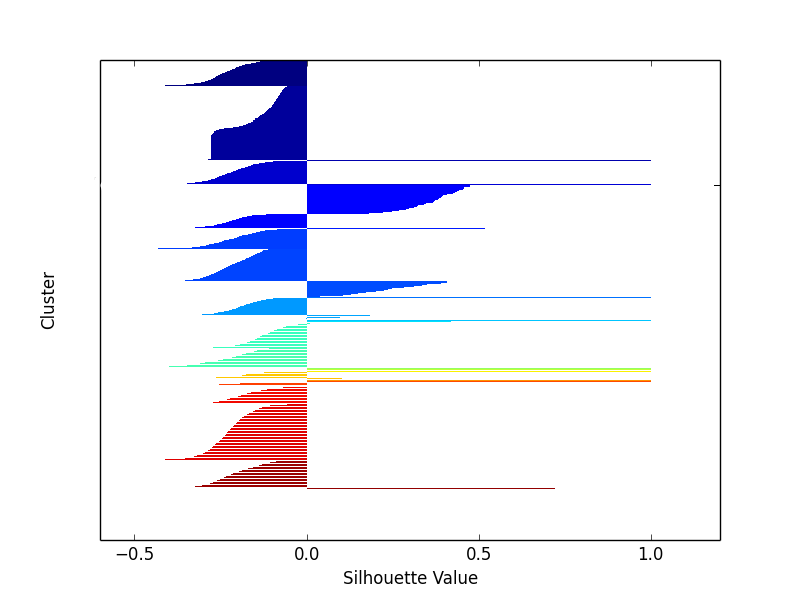
\includegraphics[scale=0.6]{KMEANS.png}
\caption{Silhouette plot for the KMeans clustering algorithm.}
\end{figure}

The results of the clustering algorithms would likely be improved with a few changes to the task. Firstly some very similar topics could be merged, as discussed above. Secondly each text could only be assigned a single topic in order to give the clusters more distinct boundaries. Lastly the algorithms would be likely to perform better if there were far less, more distinct, clusters, with more training examples for each.

\section{Conclusion}
The results discussed above show that text classification is a difficult task, particularly when there are a lot of topics to classify or cluster over. Sufficient numbers of examples must be given in order for the classifiers to gain an acceptable level of accuracy. The problem becomes more pronounced when many topics overlap or texts are assigned multiple topics, causing classifiers difficulty in finding distinguishing features for topics. Better results can be obtained when features are normalised, however different classification methods perform better with different methods of vectorisation and feature selection. Overall the best combination seemed to be a unigram TFIDF vectoriser and a linear SVM classifier. A greater number of features can give better results, however including too many features risks including irrelevant information in the final feature set.

\appendix

\clearpage

\begin{table}[H]
\begin{tabular}{l|llll}
\textbf{Topic}       & \textbf{Precision} & \textbf{Recall} & \textbf{F1-score} & \textbf{Support} \\ \hline
\textbf{acq}         & 0.95               & 0.86            & 0.9               & 718              \\
\textbf{corn}        & 0.38               & 0.05            & 0.09              & 56               \\
\textbf{crude}       & 0.82               & 0.68            & 0.74              & 189              \\
\textbf{earn}        & 0.86               & 0.98            & 0.92              & 1088             \\
\textbf{grain}       & 0.5                & 0.68            & 0.58              & 149              \\
\textbf{interest}    & 0.69               & 0.55            & 0.61              & 133              \\
\textbf{money-fx}    & 0.7                & 0.68            & 0.69              & 179              \\
\textbf{ship}        & 0.6                & 0.69            & 0.64              & 89               \\
\textbf{trade}       & 0.74               & 0.84            & 0.79              & 118              \\
\textbf{wheat}       & 0.45               & 0.14            & 0.22              & 71               \\
\textbf{avg / total} & 0.81               & 0.82            & 0.81              & 2790            
\end{tabular}
\caption {Count best classifier: MultinomialNB; per topic metrics}
\end{table}

\begin{table}[H]
\begin{tabular}{l|l}
\textbf{Accuracy}        & 0.816846 \\
\textbf{Recall macro}    & 0.614784 \\
\textbf{Recall micro}    & 0.816846 \\
\textbf{Precision macro} & 0.668779 \\
\textbf{Precision micro} & 0.816846
\end{tabular}
\caption {Count best classifier: MultinomialNB; average metrics}
\end{table}

\begin{table}[H]
\begin{tabular}{l|lll}
\textbf{Classifier}             & \textbf{Mean} & \textbf{Std. Dev.} & \textbf{Confidence Interval} \\ \hline
\textbf{GaussianNB}             & 0.549348      & 0.012712                    & {[}0.524431, 0.574264{]}     \\
\textbf{MultinomialNB}          & 0.771477      & 0.012158                    & {[}0.747648, 0.795306{]}     \\
\textbf{BernoulliNB}            & 0.599103      & 0.020672                    & {[}0.558585, 0.639621{]}     \\
\textbf{DecisionTreeClassifier} & 0.69363       & 0.018666                    & {[}0.657045, 0.730215{]}     \\
\textbf{RandomForestClassifier} & 0.740479      & 0.020325                    & {[}0.700643, 0.780315{]}     \\
\textbf{Perceptron}             & 0.751316      & 0.016738                    & {[}0.718510, 0.784123{]}     \\
\textbf{LinearSVC}              & 0.741865      & 0.013951                    & {[}0.714522, 0.769208{]}     \\
\textbf{KNeighborsClassifier}   & 0.653737      & 0.018184                    & {[}0.618097, 0.689377{]}     \\
\textbf{NearestCentroid}        & 0.670555      & 0.020061                    & {[}0.631236, 0.709874{]}    
\end{tabular}
\caption {Count: Confidence intervals for accuracy of all classifiers}
\end{table}

\clearpage

\begin{table}[H]
\begin{tabular}{l|llll}
\textbf{Topic}       & \textbf{Precision} & \textbf{Recall} & \textbf{F1-score} & \textbf{Support} \\ \hline
\textbf{acq}         & 0.95               & 0.86            & 0.9               & 718              \\
\textbf{corn}        & 0                  & 0               & 0                 & 56               \\
\textbf{crude}       & 0.76               & 0.74            & 0.75              & 189              \\
\textbf{earn}        & 0.86               & 0.98            & 0.91              & 1088             \\
\textbf{grain}       & 0.5                & 0.79            & 0.61              & 149              \\
\textbf{interest}    & 0.73               & 0.37            & 0.49              & 133              \\
\textbf{money-fx}    & 0.63               & 0.75            & 0.68              & 179              \\
\textbf{ship}        & 0.64               & 0.51            & 0.57              & 89               \\
\textbf{trade}       & 0.75               & 0.81            & 0.78              & 118              \\
\textbf{wheat}       & 0                  & 0               & 0                 & 71               \\ \hline
\textbf{avg / total} & 0.78               & 0.81            & 0.79              & 2790            
\end{tabular}
\caption {Binary best classifier: MultinomialNB; per topic metrics}
\end{table}

\begin{table}[H]
\begin{tabular}{l|l}
\textbf{Accuracy}        & 0.810753 \\
\textbf{Recall macro}    & 0.579237 \\
\textbf{Recall micro}    & 0.810753 \\
\textbf{Precision macro} & 0.581382 \\
\textbf{Precision micro} & 0.810753
\end{tabular}
\caption {Binary best classifier: MultinomialNB; average metrics}
\end{table}

\begin{table}[H]
\begin{tabular}{llll}
\textbf{Classifier}             & \textbf{Mean} & \textbf{Standard Deviation} & \textbf{Confidence Interval} \\
\textbf{GaussianNB}             & 0.549486      & 0.017148                    & {[}0.515876, 0.583096{]}     \\
\textbf{MultinomialNB}          & 0.775639      & 0.018774                    & {[}0.738841, 0.812437{]}     \\
\textbf{BernoulliNB}            & 0.399364      & 0.019681                    & {[}0.360790, 0.437938{]}     \\
\textbf{DecisionTreeClassifier} & 0.689602      & 0.022481                    & {[}0.645541, 0.733664{]}     \\
\textbf{RandomForestClassifier} & 0.740199      & 0.022583                    & {[}0.695937, 0.784462{]}     \\
\textbf{Perceptron}             & 0.735612      & 0.014251                    & {[}0.707680, 0.763543{]}     \\
\textbf{LinearSVC}              & 0.741448      & 0.016434                    & {[}0.709237, 0.773658{]}     \\
\textbf{KNeighborsClassifier}   & 0.570894      & 0.022694                    & {[}0.526414, 0.615373{]}     \\
\textbf{NearestCentroid}        & 0.714343      & 0.01706                     & {[}0.680905, 0.747781{]}    
\end{tabular}
\caption {Binary: Confidence intervals for accuracy of all classifiers}
\end{table}

\clearpage

\begin{table}[H]
\label{tab:title}
\begin{tabular}{l|llll}
\textbf{Topic}       & \textbf{Precision} & \textbf{Recall} & \textbf{F1-score} & \textbf{Support} \\ \hline
\textbf{acq}         & 0.82               & 0.98            & 0.9               & 718              \\
\textbf{corn}        & 0.39               & 0.25            & 0.3               & 56               \\
\textbf{crude}       & 0.77               & 0.75            & 0.76              & 189              \\
\textbf{earn}        & 0.98               & 0.96            & 0.97              & 1088             \\
\textbf{grain}       & 0.54               & 0.54            & 0.54              & 149              \\
\textbf{interest}    & 0.75               & 0.53            & 0.62              & 133              \\
\textbf{money-fx}    & 0.72               & 0.72            & 0.72              & 179              \\
\textbf{ship}        & 0.71               & 0.49            & 0.58              & 89               \\
\textbf{trade}       & 0.81               & 0.87            & 0.84              & 118              \\
\textbf{wheat}       & 0.45               & 0.31            & 0.37              & 71               \\ \hline
\textbf{avg / total} & 0.84               & 0.84            & 0.83              & 2790             \\
\end{tabular}
\caption {TFIDF best classifier: LinearSVC; per topic metrics}
\end{table}

\begin{table}[H]
\begin{tabular}{l|l}
\textbf{Accuracy}        & 0.841935 \\
\textbf{Recall macro}    & 0.640737 \\
\textbf{Recall micro}    & 0.841935 \\
\textbf{Precision macro} & 0.69495  \\
\textbf{Precision micro} & 0.841935
\end{tabular}
\caption {TFIDF best classifier: LinearSVC; average metrics}
\end{table}

\begin{table}[H]
\begin{tabular}{l|lll}
\textbf{Classifier}             & \textbf{Mean} & \textbf{Std. Dev.} & \textbf{Confidence Interval} \\ \hline
\textbf{GaussianNB}             & 0.550731      & 0.016708                    & {[}0.517983, 0.583478{]}     \\
\textbf{MultinomialNB}          & 0.743255      & 0.020728                    & {[}0.702627, 0.783882{]}     \\
\textbf{BernoulliNB}            & 0.399359      & 0.010567                    & {[}0.378647, 0.420071{]}     \\
\textbf{DecisionTreeClassifier} & 0.689608      & 0.015888                    & {[}0.658467, 0.720749{]}     \\
\textbf{RandomForestClassifier} & 0.742564      & 0.018824                    & {[}0.705670, 0.779458{]}     \\
\textbf{Perceptron}             & 0.71532       & 0.014534                    & {[}0.686833, 0.743808{]}     \\
\textbf{LinearSVC}              & 0.765356      & 0.011738                    & {[}0.742350, 0.788362{]}     \\
\textbf{KNeighborsClassifier}   & 0.491522      & 0.011612                    & {[}0.468762, 0.514282{]}     \\
\textbf{NearestCentroid}        & 0.715178      & 0.010247                    & {[}0.695094, 0.735261{]}    
\end{tabular}
\caption {TFIDF: Confidence intervals for accuracy of all classifiers}
\end{table}

\begin{table}[H]
\begin{tabular}{llll}
\textbf{Fold}      & \textbf{RandomForest} & \textbf{LinearSVC} & \textbf{MultinomialNB} \\ \hline
\textbf{1}         & 0.746                 & 0.779              & 0.760                  \\
\textbf{2}         & 0.733                 & 0.763              & 0.729                  \\
\textbf{3}         & 0.753                 & 0.778              & 0.769                  \\
\textbf{4}         & 0.735                 & 0.768              & 0.739                  \\
\textbf{5}         & 0.765                 & 0.777              & 0.757                  \\
\textbf{6}         & 0.773                 & 0.768              & 0.758                  \\
\textbf{7}         & 0.708                 & 0.740              & 0.713                  \\
\textbf{8}         & 0.736                 & 0.757              & 0.752                  \\
\textbf{9}         & 0.722                 & 0.754              & 0.702                  \\
\textbf{10}        & 0.755                 & 0.769              & 0.752                  \\ \hline
\textbf{Mean}      & 0.7426                & 0.7653             & 0.743                  \\ \hline
\textbf{Std. dev.} & 0.01976079171         & 0.01227508769      & 0.02196183558       
\end{tabular}
\caption {TFIDF: Per fold accuracies for three best classifiers}
\end{table}

\begin{table}[H]
\begin{tabular}{llll}
\textbf{Fold}      & \textbf{RF-SVM} & \textbf{RF-NB} & \textbf{SVM-NB} \\ \hline
\textbf{1}         & -0.033          & -0.014         & 0.019           \\
\textbf{2}         & -0.03           & 0.004          & 0.034           \\
\textbf{3}         & -0.025          & -0.016         & 0.009           \\
\textbf{4}         & -0.033          & -0.004         & 0.029           \\
\textbf{5}         & -0.012          & 0.008          & 0.020           \\
\textbf{6}         & 0.005           & 0.015          & 0.010           \\
\textbf{7}         & -0.032          & -0.005         & 0.027           \\
\textbf{8}         & -0.021          & -0.016         & 0.005           \\
\textbf{9}         & -0.032          & 0.020          & 0.052           \\
\textbf{10}        & -0.014          & 0.003          & 0.017           \\ \hline
\textbf{Mean}      & -0.0227         & -0.001         & 0.022           \\ \hline
\textbf{Std. dev.} & 0.0125          & 0.0127         & 0.0140          \\ \hline
\textbf{t-value}   & -5.7471         & -0.1241        & 5.0236          \\ \hline
\textbf{p-value}   & 0.9999          & 0.5480         & 0.9996         
\end{tabular}
\caption{TFIDF: Paired t-test for per fold accuracies of three best classifiers}
\end{table}

\clearpage

\begin{table}[h]
\begin{tabular}{l|llll}
\textbf{Topic}       & \textbf{Precision} & \textbf{Recall} & \textbf{F1-score} & \textbf{Support} \\ \hline
\textbf{acq}         & 0.83               & 0.98            & 0.9               & 718              \\
\textbf{corn}        & 0.47               & 0.12            & 0.2               & 56               \\
\textbf{crude}       & 0.8                & 0.74            & 0.77              & 189              \\
\textbf{earn}        & 0.98               & 0.96            & 0.97              & 1088             \\
\textbf{grain}       & 0.51               & 0.7             & 0.59              & 149              \\
\textbf{interest}    & 0.77               & 0.5             & 0.61              & 133              \\
\textbf{money-fx}    & 0.69               & 0.74            & 0.72              & 179              \\
\textbf{ship}        & 0.69               & 0.57            & 0.63              & 89               \\
\textbf{trade}       & 0.85               & 0.88            & 0.86              & 118              \\
\textbf{wheat}       & 0.5                & 0.14            & 0.22              & 71               \\
\textbf{avg / total} & 0.84               & 0.84            & 0.83              & 2790            
\end{tabular}
\caption {TFIDF bigrams best classifier: LinearSVC; per topic metrics}
\end{table}

\begin{table}[h]
\begin{tabular}{l|l}
\textbf{Accuracy}        & 0.844444 \\
\textbf{Recall macro}    & 0.633236 \\
\textbf{Recall micro}    & 0.844444 \\
\textbf{Precision macro} & 0.708746 \\
\textbf{Precision micro} & 0.844444
\end{tabular}
\caption {TFIDF bigrams best classifier: LinearSVC; average metrics}
\end{table}

\begin{table}[h]
\begin{tabular}{l|lll}
\textbf{Classifier}             & \textbf{Mean} & \textbf{Std. Dev.} & \textbf{Confidence Interval} \\ \hline
\textbf{GaussianNB}             & 0.690992      & 0.018064           & {[}0.655587, 0.726397{]}     \\
\textbf{MultinomialNB}          & 0.669586      & 0.016986           & {[}0.636294, 0.702879{]}     \\
\textbf{DecisionTreeClassifier} & 0.685991      & 0.01124            & {[}0.663959, 0.708022{]}     \\
\textbf{RandomForestClassifier} & 0.73311       & 0.019611           & {[}0.694674, 0.771547{]}     \\
\textbf{Perceptron}             & 0.681266      & 0.019072           & {[}0.643885, 0.718647{]}     \\
\textbf{LinearSVC}              & 0.764111      & 0.01521            & {[}0.734299, 0.793924{]}     \\
\textbf{KNeighborsClassifier}   & 0.422849      & 0.019933           & {[}0.383781, 0.461918{]}     \\
\textbf{NearestCentroid}        & 0.680293      & 0.013694           & {[}0.653453, 0.707134{]}    
\end{tabular}
\caption {TFIDF bigrams: Confidence intervals for accuracy of all classifiers}
\end{table}

\clearpage

\begin{table}[h]
\begin{tabular}{l|lllll}
\textbf{Algorithm} & \textbf{Homogeneity} & \textbf{Completeness} & \textbf{V-measure} & \textbf{ARI} & \textbf{Silhouette} \\ \hline
\textbf{KMeans}    & 0.306                & 0.292                 & 0.299              & 0.103     & -0.005           \\
\textbf{DBSCAN}    & 0.005                & 0.062                 & 0.008              & 0.001    & 0.419         \\
\textbf{Ward}      & 0.247                & 0.17                  & 0.201              & 0.029   & 0.384                    
\end{tabular}
\caption{Count: Unsupervised clustering results}
\end{table}

\begin{table}[h]
\begin{tabular}{l|ll}
             & \textbf{Training accuracy} & \textbf{Test accuracy} \\ \hline
\textbf{GMM} & 0.5                      & 0.323                 
\end{tabular}
\caption{Count: GMM clustering results}
\end{table}

\begin{table}[h]
\begin{tabular}{l|lllll}
\textbf{Algorithm} & \textbf{Homogeneity} & \textbf{Completeness} & \textbf{V-measure} & \textbf{ARI}  & \textbf{Silhouette} \\ \hline
\textbf{KMeans}    & 0.37                 & 0.378                 & 0.374              & 0.148   & -0.058          \\
\textbf{DBSCAN}    & 0.005                & 0.062                 & 0.008              & 0.001  & 0.300      \\
\textbf{Ward}      & 0.361                & 0.234                 & 0.284              & 0.043  & 0.362                    
\end{tabular}
\caption{Binary: Unsupervised clustering results}
\end{table}

\begin{table}[h]
\begin{tabular}{l|ll}
             & \textbf{Training accuracy} & \textbf{Test accuracy} \\ \hline
\textbf{GMM} & 0.389                      & 0.143                 
\end{tabular}
\caption{Binary: GMM clustering results}
\end{table}

\begin{table}[h]
\begin{tabular}{l|lllll}
\textbf{Algorithm} & \textbf{Homogeneity} & \textbf{Completeness} & \textbf{V-measure} & \textbf{ARI} & \textbf{Silhouette} \\ \hline
\textbf{KMeans}    & 0.392                & 0.39                  & 0.391              & 0.175    &   0.061    \\
\textbf{DBSCAN}    & 0.005                & 0.062                 & 0.008              & 0.001  &  0.432  \\
\textbf{Ward}      & 0.267                & 0.183                 & 0.217              & 0.023   & 0.359
\end{tabular}
\caption{TFIDF: Unsupervised clustering results}
\end{table}

\begin{table}[h]
\begin{tabular}{l|ll}
             & \textbf{Training accuracy} & \textbf{Test accuracy} \\ \hline
\textbf{GMM} & 0.348                      & 0.287                 
\end{tabular}
\caption{TFIDF: GMM clustering results}
\end{table}

\begin{table}[h]
\begin{tabular}{l|llll}
\textbf{Algorithm} & \textbf{Homogeneity} & \textbf{Completeness} & \textbf{V-measure} & \textbf{ARI} \\ \hline
\textbf{KMeans}    & 0.166                & 0.314                 & 0.217              & -0.064       \\
\textbf{DBSCAN}    & 0.005                & 0.062                 & 0.008              & 0.001        \\
\textbf{Ward}      & 0.242                & 0.167                 & 0.198              & 0.017       
\end{tabular}
\caption{TFIDF bigrams: Unsupervised clustering results}
\end{table}

\clearpage

\begin{table}[h]
\begin{tabular}{llllllll}
\textbf{Fold} & \textbf{Classifier}    & \textbf{Accuracy} & \textbf{f1-score} & \textbf{R. macro} & \textbf{R. micro} & \textbf{P. macro} & \textbf{P. micro} \\ \hline
1             & GaussianNB             & 0.551389          & 0.582172          & 0.432803              & 0.551389              & 0.416821                 & 0.551389                 \\
1             & MultinomialNB          & 0.783333          & 0.777596          & 0.574115              & 0.783333              & 0.559872                 & 0.783333                 \\
1             & BernoulliNB            & 0.625             & 0.574132          & 0.318633              & 0.625                 & 0.499196                 & 0.625                    \\
1             & DecisionTreeClassifier & 0.726389          & 0.722108          & 0.49479               & 0.726389              & 0.506527                 & 0.726389                 \\
1             & RandomForestClassifier & 0.776389          & 0.761199          & 0.498799              & 0.776389              & 0.556611                 & 0.776389                 \\
1             & Perceptron             & 0.769444          & 0.773658          & 0.541583              & 0.769444              & 0.539933                 & 0.769444                 \\
1             & LinearSVC              & 0.770833          & 0.769167          & 0.530162              & 0.770833              & 0.52373                  & 0.770833                 \\
1             & KNeighborsClassifier   & 0.686111          & 0.667624          & 0.414822              & 0.686111              & 0.541141                 & 0.686111                 \\
1             & NearestCentroid        & 0.701389          & 0.685721          & 0.576143              & 0.701389              & 0.593352                 & 0.701389                 \\
2             & GaussianNB             & 0.534722          & 0.566037          & 0.397049              & 0.534722              & 0.412183                 & 0.534722                 \\
2             & MultinomialNB          & 0.743056          & 0.733729          & 0.547385              & 0.743056              & 0.545786                 & 0.743056                 \\
2             & BernoulliNB            & 0.588889          & 0.532714          & 0.322699              & 0.588889              & 0.429885                 & 0.588889                 \\
2             & DecisionTreeClassifier & 0.668056          & 0.656846          & 0.458957              & 0.668056              & 0.438016                 & 0.668056                 \\
2             & RandomForestClassifier & 0.697222          & 0.679464          & 0.444686              & 0.697222              & 0.478304                 & 0.697222                 \\
2             & Perceptron             & 0.756944          & 0.751151          & 0.546554              & 0.756944              & 0.565361                 & 0.756944                 \\
2             & LinearSVC              & 0.7375            & 0.728213          & 0.503998              & 0.7375                & 0.501299                 & 0.7375                   \\
2             & KNeighborsClassifier   & 0.648611          & 0.622567          & 0.426295              & 0.648611              & 0.492046                 & 0.648611                 \\
2             & NearestCentroid        & 0.638889          & 0.621482          & 0.506968              & 0.638889              & 0.519516                 & 0.638889                 \\
3             & GaussianNB             & 0.536111          & 0.567208          & 0.398539              & 0.536111              & 0.41238                  & 0.536111                 \\
3             & MultinomialNB          & 0.770833          & 0.761491          & 0.543605              & 0.770833              & 0.551656                 & 0.770833                 \\
3             & BernoulliNB            & 0.611111          & 0.55252           & 0.322015              & 0.611111              & 0.434991                 & 0.611111                 \\
3             & DecisionTreeClassifier & 0.697222          & 0.691676          & 0.456919              & 0.697222              & 0.485302                 & 0.697222                 \\
3             & RandomForestClassifier & 0.738889          & 0.722484          & 0.481765              & 0.738889              & 0.505805                 & 0.738889                 \\
3             & Perceptron             & 0.741667          & 0.733728          & 0.492873              & 0.741667              & 0.52248                  & 0.741667                 \\
3             & LinearSVC              & 0.736111          & 0.734867          & 0.483142              & 0.736111              & 0.508556                 & 0.736111                 \\
3             & KNeighborsClassifier   & 0.655556          & 0.630865          & 0.396931              & 0.655556              & 0.46831                  & 0.655556                 \\
3             & NearestCentroid        & 0.672222          & 0.659302          & 0.513055              & 0.672222              & 0.562345                 & 0.672222                 \\
4             & GaussianNB             & 0.568056          & 0.602612          & 0.388427              & 0.568056              & 0.408657                 & 0.568056                 \\
4             & MultinomialNB          & 0.780556          & 0.773477          & 0.552034              & 0.780556              & 0.552992                 & 0.780556                 \\
4             & BernoulliNB            & 0.622222          & 0.562136          & 0.300926              & 0.622222              & 0.371908                 & 0.622222                 \\
4             & DecisionTreeClassifier & 0.469487          & 0.703504          & 0.464433              & 0.709722              & 0.469487                 & 0.469487                 \\
4             & RandomForestClassifier & 0.744444          & 0.728177          & 0.446617              & 0.744444              & 0.503294                 & 0.744444                 \\
4             & Perceptron             & 0.766667          & 0.758037          & 0.507746              & 0.766667              & 0.557692                 & 0.766667                 \\
4             & LinearSVC              & 0.748611          & 0.741632          & 0.472898              & 0.748611              & 0.477213                 & 0.748611                 \\
4             & KNeighborsClassifier   & 0.641667          & 0.614358          & 0.372354              & 0.641667              & 0.478842                 & 0.641667                 \\
4             & NearestCentroid        & 0.695833          & 0.684444          & 0.54                  & 0.695833              & 0.568116                 & 0.695833                 \\
5             & GaussianNB             & 0.545202          & 0.581947          & 0.371286              & 0.545202              & 0.411558                 & 0.545202                 \\
5             & MultinomialNB          & 0.773296          & 0.763271          & 0.549823              & 0.773296              & 0.56822                  & 0.773296                 \\
5             & BernoulliNB            & 0.584145          & 0.523426          & 0.285131              & 0.584145              & 0.442755                 & 0.584145                 \\
5             & DecisionTreeClassifier & 0.688456          & 0.684496          & 0.44096               & 0.688456              & 0.460391                 & 0.688456                 \\
5             & RandomForestClassifier & 0.732962          & 0.72196           & 0.486144              & 0.732962              & 0.545824                 & 0.732962                 \\
5             & Perceptron             & 0.771905          & 0.76306           & 0.550249              & 0.771905              & 0.584327                 & 0.771905                 \\
5             & LinearSVC              & 0.753825          & 0.750077          & 0.496237              & 0.753825              & 0.537412                 & 0.753825                 \\
5             & KNeighborsClassifier   & 0.638387          & 0.611483          & 0.375022              & 0.638387              & 0.562544                 & 0.638387                 \\
5             & NearestCentroid        & 0.673157          & 0.66024           & 0.521716              & 0.673157              & 0.563756                 & 0.673157
\end{tabular}
\end{table}
\begin{table}[h]
\begin{tabular}{llllllll}
\textbf{Fold} & \textbf{Classifier}    & \textbf{Accuracy} & \textbf{f1-score} & \textbf{R. macro} & \textbf{R. micro} & \textbf{P. macro} & \textbf{P. micro} \\ \hline
6             & GaussianNB             & 0.549374          & 0.572728          & 0.386945              & 0.549374              & 0.38995                  & 0.549374                 \\
6             & MultinomialNB          & 0.77886           & 0.76934           & 0.581997              & 0.77886               & 0.572883                 & 0.77886                  \\
6             & BernoulliNB            & 0.620306          & 0.563028          & 0.312879              & 0.620306              & 0.402431                 & 0.620306                 \\
6             & DecisionTreeClassifier & 0.67872           & 0.672713          & 0.444257              & 0.67872               & 0.452256                 & 0.67872                  \\
6             & RandomForestClassifier & 0.751043          & 0.734727          & 0.49644               & 0.751043              & 0.530481                 & 0.751043                 \\
6             & Perceptron             & 0.749652          & 0.743677          & 0.513018              & 0.749652              & 0.523519                 & 0.749652                 \\
6             & LinearSVC              & 0.726008          & 0.72024           & 0.471745              & 0.726008              & 0.475681                 & 0.726008                 \\
6             & KNeighborsClassifier   & 0.666203          & 0.643871          & 0.433143              & 0.666203              & 0.555221                 & 0.666203                 \\
6             & NearestCentroid        & 0.673157          & 0.65926           & 0.565734              & 0.673157              & 0.575667                 & 0.673157                 \\
7             & GaussianNB             & 0.545202          & 0.580343          & 0.403692              & 0.545202              & 0.439025                 & 0.545202                 \\
7             & MultinomialNB          & 0.770515          & 0.759405          & 0.574389              & 0.770515              & 0.580784                 & 0.770515                 \\
7             & BernoulliNB            & 0.574409          & 0.508531          & 0.28197               & 0.574409              & 0.347526                 & 0.574409                 \\
7             & DecisionTreeClassifier & 0.681502          & 0.67471           & 0.44474               & 0.681502              & 0.454962                 & 0.681502                 \\
7             & RandomForestClassifier & 0.731572          & 0.717578          & 0.470887              & 0.731572              & 0.507828                 & 0.731572                 \\
7             & Perceptron             & 0.737135          & 0.739101          & 0.512856              & 0.737135              & 0.561325                 & 0.737135                 \\
7             & LinearSVC              & 0.72879           & 0.723671          & 0.485585              & 0.72879               & 0.500854                 & 0.72879                  \\
7             & KNeighborsClassifier   & 0.62726           & 0.598942          & 0.389671              & 0.62726               & 0.486571                 & 0.62726                  \\
7             & NearestCentroid        & 0.641168          & 0.62959           & 0.486659              & 0.641168              & 0.53168                  & 0.641168                 \\
8             & GaussianNB             & 0.535466          & 0.569497          & 0.396016              & 0.535466              & 0.414505                 & 0.535466                 \\
8             & MultinomialNB          & 0.770515          & 0.761359          & 0.567133              & 0.770515              & 0.587988                 & 0.770515                 \\
8             & BernoulliNB            & 0.611961          & 0.552119          & 0.334777              & 0.611961              & 0.45114                  & 0.611961                 \\
8             & DecisionTreeClassifier & 0.674548          & 0.66662           & 0.448723              & 0.674548              & 0.471579                 & 0.674548                 \\
8             & RandomForestClassifier & 0.727399          & 0.712402          & 0.496846              & 0.727399              & 0.5267                   & 0.727399                 \\
8             & Perceptron             & 0.721836          & 0.722096          & 0.51057               & 0.721836              & 0.531204                 & 0.721836                 \\
8             & LinearSVC              & 0.734353          & 0.730732          & 0.503097              & 0.734353              & 0.519537                 & 0.734353                 \\
8             & KNeighborsClassifier   & 0.632823          & 0.608493          & 0.399435              & 0.632823              & 0.455618                 & 0.632823                 \\
8             & NearestCentroid        & 0.688456          & 0.677896          & 0.556376              & 0.688456              & 0.597948                 & 0.688456                 \\
9             & GaussianNB             & 0.553547          & 0.586404          & 0.378723              & 0.553547              & 0.423193                 & 0.553547                 \\
9             & MultinomialNB          & 0.757997          & 0.746291          & 0.55035               & 0.757997              & 0.575103                 & 0.757997                 \\
9             & BernoulliNB            & 0.563282          & 0.496145          & 0.270662              & 0.563282              & 0.334035                 & 0.563282                 \\
9             & DecisionTreeClassifier & 0.691238          & 0.683859          & 0.467964              & 0.691238              & 0.492514                 & 0.691238                 \\
9             & RandomForestClassifier & 0.741307          & 0.717852          & 0.493256              & 0.741307              & 0.53655                  & 0.741307                 \\
9             & Perceptron             & 0.731572          & 0.722581          & 0.492904              & 0.731572              & 0.519828                 & 0.731572                 \\
9             & LinearSVC              & 0.727399          & 0.719866          & 0.474851              & 0.727399              & 0.494351                 & 0.727399                 \\
9             & KNeighborsClassifier   & 0.670376          & 0.641886          & 0.415296              & 0.670376              & 0.514312                 & 0.670376                 \\
9             & NearestCentroid        & 0.656467          & 0.645228          & 0.543732              & 0.656467              & 0.561429                 & 0.656467                 \\
10            & GaussianNB             & 0.574409          & 0.603768          & 0.428989              & 0.574409              & 0.425459                 & 0.574409                 \\
10            & MultinomialNB          & 0.785814          & 0.776189          & 0.570395              & 0.785814              & 0.563761                 & 0.785814                 \\
10            & BernoulliNB            & 0.589708          & 0.531048          & 0.26786               & 0.589708              & 0.378928                 & 0.589708                 \\
10            & DecisionTreeClassifier & 0.720445          & 0.71671           & 0.468791              & 0.720445              & 0.487127                 & 0.720445                 \\
10            & RandomForestClassifier & 0.763561          & 0.754408          & 0.524115              & 0.763561              & 0.554671                 & 0.763561                 \\
10            & Perceptron             & 0.766342          & 0.765981          & 0.529979              & 0.766342              & 0.565764                 & 0.766342                 \\
10            & LinearSVC              & 0.755216          & 0.753022          & 0.523457              & 0.755216              & 0.536058                 & 0.755216                 \\
10            & KNeighborsClassifier   & 0.670376          & 0.648937          & 0.405295              & 0.670376              & 0.507075                 & 0.670376                 \\
10            & NearestCentroid        & 0.664812          & 0.652596          & 0.506418              & 0.664812              & 0.554937                 & 0.664812                
\end{tabular}
\caption{Count vectoriser metric averages for each fold for each classifier}
\end{table}

\begin{table}[h]
\begin{tabular}{lllllll}
\textbf{Fold} & \textbf{Classifier}    & \textbf{Topics} & \textbf{precision} & \textbf{recall} & \textbf{f1-score} & \textbf{support} \\ \hline
1             & GaussianNB             & acq             & 0.69               & 0.58            & 0.63              & 175              \\
1             & GaussianNB             & corn            & 0.06               & 0.29            & 0.1               & 17               \\
1             & GaussianNB             & crude           & 0.46               & 0.62            & 0.53              & 39               \\
1             & GaussianNB             & earn            & 0.81               & 0.67            & 0.74              & 297              \\
1             & GaussianNB             & grain           & 0.23               & 0.17            & 0.19              & 41               \\
1             & GaussianNB             & interest        & 0.27               & 0.52            & 0.36              & 23               \\
1             & GaussianNB             & money-fx        & 0.53               & 0.32            & 0.4               & 56               \\
1             & GaussianNB             & ship            & 0.4                & 0.4             & 0.4               & 20               \\
1             & GaussianNB             & trade           & 0.55               & 0.47            & 0.51              & 34               \\
1             & GaussianNB             & wheat           & 0.17               & 0.28            & 0.21              & 18               \\
1             & MultinomialNB          & acq             & 0.89               & 0.86            & 0.88              & 175              \\
1             & MultinomialNB          & corn            & 0                  & 0               & 0                 & 17               \\
1             & MultinomialNB          & crude           & 0.83               & 0.77            & 0.8               & 39               \\
1             & MultinomialNB          & earn            & 0.89               & 0.94            & 0.91              & 297              \\
1             & MultinomialNB          & grain           & 0.32               & 0.34            & 0.33              & 41               \\
1             & MultinomialNB          & interest        & 0.5                & 0.74            & 0.6               & 23               \\
1             & MultinomialNB          & money-fx        & 0.77               & 0.61            & 0.68              & 56               \\
1             & MultinomialNB          & ship            & 0.71               & 0.75            & 0.73              & 20               \\
1             & MultinomialNB          & trade           & 0.68               & 0.74            & 0.7               & 34               \\
1             & MultinomialNB          & wheat           & 0                  & 0               & 0                 & 18               \\
1             & BernoulliNB            & acq             & 0.69               & 0.56            & 0.62              & 175              \\
1             & BernoulliNB            & corn            & 0                  & 0               & 0                 & 17               \\
1             & BernoulliNB            & crude           & 0.73               & 0.49            & 0.58              & 39               \\
1             & BernoulliNB            & earn            & 0.6                & 0.95            & 0.74              & 297              \\
1             & BernoulliNB            & grain           & 0.46               & 0.44            & 0.45              & 41               \\
1             & BernoulliNB            & interest        & 1                  & 0.04            & 0.08              & 23               \\
1             & BernoulliNB            & money-fx        & 0.69               & 0.32            & 0.44              & 56               \\
1             & BernoulliNB            & ship            & 0                  & 0               & 0                 & 20               \\
1             & BernoulliNB            & trade           & 0.81               & 0.38            & 0.52              & 34               \\
1             & BernoulliNB            & wheat           & 0                  & 0               & 0                 & 18               \\
1             & DecisionTreeClassifier & acq             & 0.72               & 0.86            & 0.78              & 175              \\
1             & DecisionTreeClassifier & corn            & 0.12               & 0.12            & 0.12              & 17               \\
1             & DecisionTreeClassifier & crude           & 0.73               & 0.69            & 0.71              & 39               \\
1             & DecisionTreeClassifier & earn            & 0.92               & 0.88            & 0.9               & 297              \\
1             & DecisionTreeClassifier & grain           & 0.2                & 0.15            & 0.17              & 41               \\
1             & DecisionTreeClassifier & interest        & 0.34               & 0.48            & 0.4               & 23               \\
1             & DecisionTreeClassifier & money-fx        & 0.65               & 0.57            & 0.61              & 56               \\
1             & DecisionTreeClassifier & ship            & 0.56               & 0.5             & 0.53              & 20               \\
1             & DecisionTreeClassifier & trade           & 0.76               & 0.65            & 0.7               & 34               \\
1             & DecisionTreeClassifier & wheat           & 0.07               & 0.06            & 0.06              & 18               \\
1             & RandomForestClassifier & acq             & 0.75               & 0.98            & 0.85              & 175              \\
1             & RandomForestClassifier & corn            & 0                  & 0               & 0                 & 17               \\
1             & RandomForestClassifier & crude           & 0.69               & 0.56            & 0.62              & 39               \\
1             & RandomForestClassifier & earn            & 0.94               & 0.91            & 0.93              & 297              \\\end{tabular}
\end{table}
\begin{table}[h]
\begin{tabular}{lllllll}
\textbf{Fold} & \textbf{Classifier}    & \textbf{Topics} & \textbf{precision} & \textbf{recall} & \textbf{f1-score} & \textbf{support} \\ \hline
1             & RandomForestClassifier & grain           & 0.31               & 0.37            & 0.34              & 41               \\
1             & RandomForestClassifier & interest        & 0.58               & 0.48            & 0.52              & 23               \\
1             & RandomForestClassifier & money-fx        & 0.75               & 0.68            & 0.71              & 56               \\
1             & RandomForestClassifier & ship            & 0.75               & 0.3             & 0.43              & 20               \\
1             & RandomForestClassifier & trade           & 0.8                & 0.71            & 0.75              & 34               \\
1             & RandomForestClassifier & wheat           & 0                  & 0               & 0                 & 18               \\
1             & Perceptron             & acq             & 0.93               & 0.85            & 0.89              & 175              \\
1             & Perceptron             & corn            & 0.07               & 0.06            & 0.06              & 17               \\
1             & Perceptron             & crude           & 0.42               & 0.87            & 0.57              & 39               \\
1             & Perceptron             & earn            & 0.96               & 0.93            & 0.95              & 297              \\
1             & Perceptron             & grain           & 0.23               & 0.17            & 0.2               & 41               \\
1             & Perceptron             & interest        & 0.67               & 0.43            & 0.53              & 23               \\
1             & Perceptron             & money-fx        & 0.69               & 0.73            & 0.71              & 56               \\
1             & Perceptron             & ship            & 0.53               & 0.5             & 0.51              & 20               \\
1             & Perceptron             & trade           & 0.77               & 0.71            & 0.74              & 34               \\
1             & Perceptron             & wheat           & 0.12               & 0.17            & 0.14              & 18               \\
1             & LinearSVC              & acq             & 0.81               & 0.93            & 0.86              & 175              \\
1             & LinearSVC              & corn            & 0                  & 0               & 0                 & 17               \\
1             & LinearSVC              & crude           & 0.74               & 0.74            & 0.74              & 39               \\
1             & LinearSVC              & earn            & 0.98               & 0.92            & 0.95              & 297              \\
1             & LinearSVC              & grain           & 0.15               & 0.12            & 0.14              & 41               \\
1             & LinearSVC              & interest        & 0.37               & 0.48            & 0.42              & 23               \\
1             & LinearSVC              & money-fx        & 0.7                & 0.59            & 0.64              & 56               \\
1             & LinearSVC              & ship            & 0.64               & 0.7             & 0.67              & 20               \\
1             & LinearSVC              & trade           & 0.81               & 0.76            & 0.79              & 34               \\
1             & LinearSVC              & wheat           & 0.04               & 0.06            & 0.05              & 18               \\
1             & KNeighborsClassifier   & acq             & 0.67               & 0.73            & 0.7               & 175              \\
1             & KNeighborsClassifier   & corn            & 0.2                & 0.12            & 0.15              & 17               \\
1             & KNeighborsClassifier   & crude           & 0.8                & 0.51            & 0.62              & 39               \\
1             & KNeighborsClassifier   & earn            & 0.82               & 0.92            & 0.87              & 297              \\
1             & KNeighborsClassifier   & grain           & 0.26               & 0.27            & 0.26              & 41               \\
1             & KNeighborsClassifier   & interest        & 0.28               & 0.52            & 0.36              & 23               \\
1             & KNeighborsClassifier   & money-fx        & 0.63               & 0.59            & 0.61              & 56               \\
1             & KNeighborsClassifier   & ship            & 1                  & 0.05            & 0.1               & 20               \\
1             & KNeighborsClassifier   & trade           & 0.75               & 0.44            & 0.56              & 34               \\
1             & KNeighborsClassifier   & wheat           & 0                  & 0               & 0                 & 18               \\
1             & NearestCentroid        & acq             & 0.72               & 0.81            & 0.76              & 175              \\
1             & NearestCentroid        & corn            & 0.33               & 0.35            & 0.34              & 17               \\
1             & NearestCentroid        & crude           & 0.55               & 0.69            & 0.61              & 39               \\
1             & NearestCentroid        & earn            & 0.77               & 0.82            & 0.8               & 297              \\
1             & NearestCentroid        & grain           & 0.42               & 0.12            & 0.19              & 41               \\
1             & NearestCentroid        & interest        & 0.57               & 0.7             & 0.63              & 23               \\
1             & NearestCentroid        & money-fx        & 0.73               & 0.34            & 0.46              & 56               \\
1             & NearestCentroid        & ship            & 0.67               & 0.7             & 0.68              & 20               \\
1             & NearestCentroid        & trade           & 0.72               & 0.68            & 0.7               & 34               \\
1             & NearestCentroid        & wheat           & 0.45               & 0.56            & 0.5               & 18               \end{tabular}
\end{table}
\begin{table}[h]
\begin{tabular}{lllllll}
\textbf{Fold} & \textbf{Classifier}    & \textbf{Topics} & \textbf{precision} & \textbf{recall} & \textbf{f1-score} & \textbf{support} \\ \hline
2             & GaussianNB             & acq             & 0.65               & 0.61            & 0.63              & 160              \\
2             & GaussianNB             & corn            & 0.02               & 0.14            & 0.04              & 14               \\
2             & GaussianNB             & crude           & 0.57               & 0.55            & 0.56              & 49               \\
2             & GaussianNB             & earn            & 0.83               & 0.68            & 0.75              & 268              \\
2             & GaussianNB             & grain           & 0.22               & 0.17            & 0.19              & 48               \\
2             & GaussianNB             & interest        & 0.41               & 0.5             & 0.45              & 44               \\
2             & GaussianNB             & money-fx        & 0.47               & 0.31            & 0.38              & 61               \\
2             & GaussianNB             & ship            & 0.33               & 0.41            & 0.37              & 17               \\
2             & GaussianNB             & trade           & 0.53               & 0.51            & 0.52              & 35               \\
2             & GaussianNB             & wheat           & 0.08               & 0.08            & 0.08              & 24               \\
2             & MultinomialNB          & acq             & 0.89               & 0.84            & 0.86              & 160              \\
2             & MultinomialNB          & corn            & 0                  & 0               & 0                 & 14               \\
2             & MultinomialNB          & crude           & 0.85               & 0.69            & 0.76              & 49               \\
2             & MultinomialNB          & earn            & 0.85               & 0.94            & 0.9               & 268              \\
2             & MultinomialNB          & grain           & 0.35               & 0.33            & 0.34              & 48               \\
2             & MultinomialNB          & interest        & 0.59               & 0.52            & 0.55              & 44               \\
2             & MultinomialNB          & money-fx        & 0.58               & 0.52            & 0.55              & 61               \\
2             & MultinomialNB          & ship            & 0.57               & 0.71            & 0.63              & 17               \\
2             & MultinomialNB          & trade           & 0.64               & 0.83            & 0.73              & 35               \\
2             & MultinomialNB          & wheat           & 0.13               & 0.08            & 0.1               & 24               \\
2             & BernoulliNB            & acq             & 0.63               & 0.54            & 0.58              & 160              \\
2             & BernoulliNB            & corn            & 0                  & 0               & 0                 & 14               \\
2             & BernoulliNB            & crude           & 0.85               & 0.45            & 0.59              & 49               \\
2             & BernoulliNB            & earn            & 0.57               & 0.96            & 0.72              & 268              \\
2             & BernoulliNB            & grain           & 0.53               & 0.42            & 0.47              & 48               \\
2             & BernoulliNB            & interest        & 0.6                & 0.07            & 0.12              & 44               \\
2             & BernoulliNB            & money-fx        & 0.5                & 0.28            & 0.36              & 61               \\
2             & BernoulliNB            & ship            & 0                  & 0               & 0                 & 17               \\
2             & BernoulliNB            & trade           & 0.62               & 0.51            & 0.56              & 35               \\
2             & BernoulliNB            & wheat           & 0                  & 0               & 0                 & 24               \\
2             & DecisionTreeClassifier & acq             & 0.68               & 0.82            & 0.74              & 160              \\
2             & DecisionTreeClassifier & corn            & 0.12               & 0.14            & 0.13              & 14               \\
2             & DecisionTreeClassifier & crude           & 0.65               & 0.63            & 0.64              & 49               \\
2             & DecisionTreeClassifier & earn            & 0.92               & 0.88            & 0.9               & 268              \\
2             & DecisionTreeClassifier & grain           & 0.14               & 0.08            & 0.11              & 48               \\
2             & DecisionTreeClassifier & interest        & 0.46               & 0.55            & 0.5               & 44               \\
2             & DecisionTreeClassifier & money-fx        & 0.48               & 0.34            & 0.4               & 61               \\
2             & DecisionTreeClassifier & ship            & 0.33               & 0.41            & 0.37              & 17               \\
2             & DecisionTreeClassifier & trade           & 0.53               & 0.69            & 0.6               & 35               \\
2             & DecisionTreeClassifier & wheat           & 0.06               & 0.04            & 0.05              & 24               \\
2             & RandomForestClassifier & acq             & 0.66               & 0.95            & 0.78              & 160              \\
2             & RandomForestClassifier & corn            & 0                  & 0               & 0                 & 14               \\
2             & RandomForestClassifier & crude           & 0.76               & 0.53            & 0.63              & 49               \\
2             & RandomForestClassifier & earn            & 0.92               & 0.87            & 0.89              & 268              \\\end{tabular}
\end{table}
\begin{table}[h]
\begin{tabular}{lllllll}
\textbf{Fold} & \textbf{Classifier}    & \textbf{Topics} & \textbf{precision} & \textbf{recall} & \textbf{f1-score} & \textbf{support} \\ \hline
2             & RandomForestClassifier & grain           & 0.33               & 0.33            & 0.33              & 48               \\
2             & RandomForestClassifier & interest        & 0.53               & 0.36            & 0.43              & 44               \\
2             & RandomForestClassifier & money-fx        & 0.52               & 0.52            & 0.52              & 61               \\
2             & RandomForestClassifier & ship            & 0.3                & 0.18            & 0.22              & 17               \\
2             & RandomForestClassifier & trade           & 0.61               & 0.66            & 0.63              & 35               \\
2             & RandomForestClassifier & wheat           & 0.14               & 0.04            & 0.06              & 24               \\
2             & Perceptron             & acq             & 0.77               & 0.96            & 0.85              & 160              \\
2             & Perceptron             & corn            & 0.1                & 0.21            & 0.14              & 14               \\
2             & Perceptron             & crude           & 0.81               & 0.61            & 0.7               & 49               \\
2             & Perceptron             & earn            & 0.98               & 0.93            & 0.96              & 268              \\
2             & Perceptron             & grain           & 0.3                & 0.19            & 0.23              & 48               \\
2             & Perceptron             & interest        & 0.83               & 0.43            & 0.57              & 44               \\
2             & Perceptron             & money-fx        & 0.64               & 0.67            & 0.66              & 61               \\
2             & Perceptron             & ship            & 0.53               & 0.59            & 0.56              & 17               \\
2             & Perceptron             & trade           & 0.64               & 0.83            & 0.73              & 35               \\
2             & Perceptron             & wheat           & 0.05               & 0.04            & 0.05              & 24               \\
2             & LinearSVC              & acq             & 0.76               & 0.94            & 0.84              & 160              \\
2             & LinearSVC              & corn            & 0                  & 0               & 0                 & 14               \\
2             & LinearSVC              & crude           & 0.76               & 0.63            & 0.69              & 49               \\
2             & LinearSVC              & earn            & 0.97               & 0.93            & 0.95              & 268              \\
2             & LinearSVC              & grain           & 0.22               & 0.15            & 0.18              & 48               \\
2             & LinearSVC              & interest        & 0.57               & 0.61            & 0.59              & 44               \\
2             & LinearSVC              & money-fx        & 0.64               & 0.46            & 0.53              & 61               \\
2             & LinearSVC              & ship            & 0.4                & 0.47            & 0.43              & 17               \\
2             & LinearSVC              & trade           & 0.64               & 0.8             & 0.71              & 35               \\
2             & LinearSVC              & wheat           & 0.06               & 0.04            & 0.05              & 24               \\
2             & KNeighborsClassifier   & acq             & 0.61               & 0.64            & 0.62              & 160              \\
2             & KNeighborsClassifier   & corn            & 0.17               & 0.07            & 0.1               & 14               \\
2             & KNeighborsClassifier   & crude           & 0.82               & 0.47            & 0.6               & 49               \\
2             & KNeighborsClassifier   & earn            & 0.73               & 0.91            & 0.81              & 268              \\
2             & KNeighborsClassifier   & grain           & 0.46               & 0.48            & 0.47              & 48               \\
2             & KNeighborsClassifier   & interest        & 0.52               & 0.68            & 0.59              & 44               \\
2             & KNeighborsClassifier   & money-fx        & 0.56               & 0.41            & 0.47              & 61               \\
2             & KNeighborsClassifier   & ship            & 0.4                & 0.12            & 0.18              & 17               \\
2             & KNeighborsClassifier   & trade           & 0.65               & 0.49            & 0.56              & 35               \\
2             & KNeighborsClassifier   & wheat           & 0                  & 0               & 0                 & 24               \\
2             & NearestCentroid        & acq             & 0.65               & 0.71            & 0.68              & 160              \\
2             & NearestCentroid        & corn            & 0.17               & 0.29            & 0.22              & 14               \\
2             & NearestCentroid        & crude           & 0.65               & 0.53            & 0.58              & 49               \\
2             & NearestCentroid        & earn            & 0.73               & 0.82            & 0.77              & 268              \\
2             & NearestCentroid        & grain           & 0.38               & 0.12            & 0.19              & 48               \\
2             & NearestCentroid        & interest        & 0.56               & 0.64            & 0.6               & 44               \\
2             & NearestCentroid        & money-fx        & 0.68               & 0.28            & 0.4               & 61               \\
2             & NearestCentroid        & ship            & 0.43               & 0.59            & 0.5               & 17               \\
2             & NearestCentroid        & trade           & 0.62               & 0.8             & 0.7               & 35               \\
2             & NearestCentroid        & wheat           & 0.32               & 0.29            & 0.3               & 24               \\\end{tabular}
\end{table}
\begin{table}[h]
\begin{tabular}{lllllll}
\textbf{Fold} & \textbf{Classifier}    & \textbf{Topics} & \textbf{precision} & \textbf{recall} & \textbf{f1-score} & \textbf{support} \\ \hline
3             & GaussianNB             & acq             & 0.68               & 0.6             & 0.64              & 169              \\
3             & GaussianNB             & corn            & 0.06               & 0.26            & 0.1               & 23               \\
3             & GaussianNB             & crude           & 0.44               & 0.54            & 0.49              & 35               \\
3             & GaussianNB             & earn            & 0.81               & 0.67            & 0.73              & 288              \\
3             & GaussianNB             & grain           & 0.22               & 0.21            & 0.21              & 38               \\
3             & GaussianNB             & interest        & 0.29               & 0.4             & 0.34              & 35               \\
3             & GaussianNB             & money-fx        & 0.47               & 0.27            & 0.34              & 59               \\
3             & GaussianNB             & ship            & 0.43               & 0.37            & 0.4               & 27               \\
3             & GaussianNB             & trade           & 0.64               & 0.53            & 0.58              & 30               \\
3             & GaussianNB             & wheat           & 0.08               & 0.12            & 0.1               & 16               \\
3             & MultinomialNB          & acq             & 0.95               & 0.84            & 0.89              & 169              \\
3             & MultinomialNB          & corn            & 0                  & 0               & 0                 & 23               \\
3             & MultinomialNB          & crude           & 0.77               & 0.69            & 0.73              & 35               \\
3             & MultinomialNB          & earn            & 0.86               & 0.97            & 0.91              & 288              \\
3             & MultinomialNB          & grain           & 0.33               & 0.5             & 0.4               & 38               \\
3             & MultinomialNB          & interest        & 0.56               & 0.54            & 0.55              & 35               \\
3             & MultinomialNB          & money-fx        & 0.65               & 0.58            & 0.61              & 59               \\
3             & MultinomialNB          & ship            & 0.62               & 0.56            & 0.59              & 27               \\
3             & MultinomialNB          & trade           & 0.77               & 0.77            & 0.77              & 30               \\
3             & MultinomialNB          & wheat           & 0                  & 0               & 0                 & 16               \\
3             & BernoulliNB            & acq             & 0.68               & 0.55            & 0.61              & 169              \\
3             & BernoulliNB            & corn            & 0                  & 0               & 0                 & 23               \\
3             & BernoulliNB            & crude           & 0.68               & 0.49            & 0.57              & 35               \\
3             & BernoulliNB            & earn            & 0.6                & 0.97            & 0.74              & 288              \\
3             & BernoulliNB            & grain           & 0.38               & 0.37            & 0.37              & 38               \\
3             & BernoulliNB            & interest        & 0.67               & 0.06            & 0.11              & 35               \\
3             & BernoulliNB            & money-fx        & 0.59               & 0.39            & 0.47              & 59               \\
3             & BernoulliNB            & ship            & 0                  & 0               & 0                 & 27               \\
3             & BernoulliNB            & trade           & 0.75               & 0.4             & 0.52              & 30               \\
3             & BernoulliNB            & wheat           & 0                  & 0               & 0                 & 16               \\
3             & DecisionTreeClassifier & acq             & 0.7                & 0.83            & 0.76              & 169              \\
3             & DecisionTreeClassifier & corn            & 0.17               & 0.13            & 0.15              & 23               \\
3             & DecisionTreeClassifier & crude           & 0.65               & 0.63            & 0.64              & 35               \\
3             & DecisionTreeClassifier & earn            & 0.91               & 0.89            & 0.9               & 288              \\
3             & DecisionTreeClassifier & grain           & 0.2                & 0.21            & 0.2               & 38               \\
3             & DecisionTreeClassifier & interest        & 0.44               & 0.43            & 0.43              & 35               \\
3             & DecisionTreeClassifier & money-fx        & 0.61               & 0.53            & 0.56              & 59               \\
3             & DecisionTreeClassifier & ship            & 0.5                & 0.26            & 0.34              & 27               \\
3             & DecisionTreeClassifier & trade           & 0.69               & 0.67            & 0.68              & 30               \\
3             & DecisionTreeClassifier & wheat           & 0                  & 0               & 0                 & 16               \\
3             & RandomForestClassifier & acq             & 0.72               & 0.95            & 0.82              & 169              \\
3             & RandomForestClassifier & corn            & 0                  & 0               & 0                 & 23               \\
3             & RandomForestClassifier & crude           & 0.72               & 0.51            & 0.6               & 35               \\
3             & RandomForestClassifier & earn            & 0.94               & 0.9             & 0.92              & 288              \\\end{tabular}
\end{table}
\begin{table}[h]
\begin{tabular}{lllllll}
\textbf{Fold} & \textbf{Classifier}    & \textbf{Topics} & \textbf{precision} & \textbf{recall} & \textbf{f1-score} & \textbf{support} \\ \hline
3             & RandomForestClassifier & grain           & 0.35               & 0.45            & 0.39              & 38               \\
3             & RandomForestClassifier & interest        & 0.48               & 0.37            & 0.42              & 35               \\
3             & RandomForestClassifier & money-fx        & 0.63               & 0.53            & 0.57              & 59               \\
3             & RandomForestClassifier & ship            & 0.62               & 0.37            & 0.47              & 27               \\
3             & RandomForestClassifier & trade           & 0.59               & 0.73            & 0.66              & 30               \\
3             & RandomForestClassifier & wheat           & 0                  & 0               & 0                 & 16               \\
3             & Perceptron             & acq             & 0.77               & 0.91            & 0.84              & 169              \\
3             & Perceptron             & corn            & 0.15               & 0.09            & 0.11              & 23               \\
3             & Perceptron             & crude           & 0.7                & 0.66            & 0.68              & 35               \\
3             & Perceptron             & earn            & 0.97               & 0.91            & 0.94              & 288              \\
3             & Perceptron             & grain           & 0.22               & 0.18            & 0.2               & 38               \\
3             & Perceptron             & interest        & 0.55               & 0.17            & 0.26              & 35               \\
3             & Perceptron             & money-fx        & 0.56               & 0.75            & 0.64              & 59               \\
3             & Perceptron             & ship            & 0.57               & 0.63            & 0.6               & 27               \\
3             & Perceptron             & trade           & 0.71               & 0.57            & 0.63              & 30               \\
3             & Perceptron             & wheat           & 0.04               & 0.06            & 0.05              & 16               \\
3             & LinearSVC              & acq             & 0.78               & 0.92            & 0.85              & 169              \\
3             & LinearSVC              & corn            & 0.11               & 0.04            & 0.06              & 23               \\
3             & LinearSVC              & crude           & 0.7                & 0.66            & 0.68              & 35               \\
3             & LinearSVC              & earn            & 0.97               & 0.92            & 0.94              & 288              \\
3             & LinearSVC              & grain           & 0.21               & 0.29            & 0.24              & 38               \\
3             & LinearSVC              & interest        & 0.42               & 0.43            & 0.42              & 35               \\
3             & LinearSVC              & money-fx        & 0.62               & 0.49            & 0.55              & 59               \\
3             & LinearSVC              & ship            & 0.57               & 0.48            & 0.52              & 27               \\
3             & LinearSVC              & trade           & 0.72               & 0.6             & 0.65              & 30               \\
3             & LinearSVC              & wheat           & 0                  & 0               & 0                 & 16               \\
3             & KNeighborsClassifier   & acq             & 0.65               & 0.7             & 0.68              & 169              \\
3             & KNeighborsClassifier   & corn            & 0                  & 0               & 0                 & 23               \\
3             & KNeighborsClassifier   & crude           & 0.78               & 0.4             & 0.53              & 35               \\
3             & KNeighborsClassifier   & earn            & 0.77               & 0.91            & 0.83              & 288              \\
3             & KNeighborsClassifier   & grain           & 0.31               & 0.32            & 0.31              & 38               \\
3             & KNeighborsClassifier   & interest        & 0.38               & 0.54            & 0.45              & 35               \\
3             & KNeighborsClassifier   & money-fx        & 0.58               & 0.47            & 0.52              & 59               \\
3             & KNeighborsClassifier   & ship            & 0.67               & 0.22            & 0.33              & 27               \\
3             & KNeighborsClassifier   & trade           & 0.55               & 0.4             & 0.46              & 30               \\
3             & KNeighborsClassifier   & wheat           & 0                  & 0               & 0                 & 16               \\
3             & NearestCentroid        & acq             & 0.7                & 0.78            & 0.74              & 169              \\
3             & NearestCentroid        & corn            & 0.5                & 0.3             & 0.38              & 23               \\
3             & NearestCentroid        & crude           & 0.5                & 0.4             & 0.44              & 35               \\
3             & NearestCentroid        & earn            & 0.75               & 0.83            & 0.78              & 288              \\
3             & NearestCentroid        & grain           & 0.52               & 0.29            & 0.37              & 38               \\
3             & NearestCentroid        & interest        & 0.42               & 0.46            & 0.44              & 35               \\
3             & NearestCentroid        & money-fx        & 0.72               & 0.36            & 0.48              & 59               \\
3             & NearestCentroid        & ship            & 0.58               & 0.7             & 0.63              & 27               \\
3             & NearestCentroid        & trade           & 0.64               & 0.7             & 0.67              & 30               \\
3             & NearestCentroid        & wheat           & 0.29               & 0.31            & 0.3               & 16               \\\end{tabular}
\end{table}
\begin{table}[h]
\begin{tabular}{lllllll}
\textbf{Fold} & \textbf{Classifier}    & \textbf{Topics} & \textbf{precision} & \textbf{recall} & \textbf{f1-score} & \textbf{support} \\ \hline
4             & GaussianNB             & acq             & 0.75               & 0.65            & 0.69              & 172              \\
4             & GaussianNB             & corn            & 0.03               & 0.23            & 0.06              & 13               \\
4             & GaussianNB             & crude           & 0.49               & 0.48            & 0.48              & 42               \\
4             & GaussianNB             & earn            & 0.84               & 0.73            & 0.79              & 301              \\
4             & GaussianNB             & grain           & 0.22               & 0.17            & 0.19              & 48               \\
4             & GaussianNB             & interest        & 0.39               & 0.3             & 0.34              & 30               \\
4             & GaussianNB             & money-fx        & 0.3                & 0.28            & 0.29              & 39               \\
4             & GaussianNB             & ship            & 0.36               & 0.47            & 0.41              & 17               \\
4             & GaussianNB             & trade           & 0.58               & 0.41            & 0.48              & 34               \\
4             & GaussianNB             & wheat           & 0.12               & 0.17            & 0.14              & 24               \\
4             & MultinomialNB          & acq             & 0.93               & 0.88            & 0.9               & 172              \\
4             & MultinomialNB          & corn            & 0                  & 0               & 0                 & 13               \\
4             & MultinomialNB          & crude           & 0.76               & 0.74            & 0.75              & 42               \\
4             & MultinomialNB          & earn            & 0.89               & 0.96            & 0.92              & 301              \\
4             & MultinomialNB          & grain           & 0.33               & 0.35            & 0.34              & 48               \\
4             & MultinomialNB          & interest        & 0.58               & 0.47            & 0.52              & 30               \\
4             & MultinomialNB          & money-fx        & 0.62               & 0.54            & 0.58              & 39               \\
4             & MultinomialNB          & ship            & 0.64               & 0.82            & 0.72              & 17               \\
4             & MultinomialNB          & trade           & 0.79               & 0.76            & 0.78              & 34               \\
4             & MultinomialNB          & wheat           & 0                  & 0               & 0                 & 24               \\
4             & BernoulliNB            & acq             & 0.64               & 0.53            & 0.58              & 172              \\
4             & BernoulliNB            & corn            & 0                  & 0               & 0                 & 13               \\
4             & BernoulliNB            & crude           & 0.63               & 0.29            & 0.39              & 42               \\
4             & BernoulliNB            & earn            & 0.62               & 0.98            & 0.76              & 301              \\
4             & BernoulliNB            & grain           & 0.62               & 0.5             & 0.55              & 48               \\
4             & BernoulliNB            & interest        & 0                  & 0               & 0                 & 30               \\
4             & BernoulliNB            & money-fx        & 0.5                & 0.36            & 0.42              & 39               \\
4             & BernoulliNB            & ship            & 0                  & 0               & 0                 & 17               \\
4             & BernoulliNB            & trade           & 0.71               & 0.35            & 0.47              & 34               \\
4             & BernoulliNB            & wheat           & 0                  & 0               & 0                 & 24               \\
4             & DecisionTreeClassifier & acq             & 0.7                & 0.88            & 0.78              & 172              \\
4             & DecisionTreeClassifier & corn            & 0                  & 0               & 0                 & 13               \\
4             & DecisionTreeClassifier & crude           & 0.69               & 0.64            & 0.67              & 42               \\
4             & DecisionTreeClassifier & earn            & 0.94               & 0.87            & 0.91              & 301              \\
4             & DecisionTreeClassifier & grain           & 0.24               & 0.21            & 0.22              & 48               \\
4             & DecisionTreeClassifier & interest        & 0.43               & 0.33            & 0.38              & 30               \\
4             & DecisionTreeClassifier & money-fx        & 0.44               & 0.38            & 0.41              & 39               \\
4             & DecisionTreeClassifier & ship            & 0.56               & 0.59            & 0.57              & 17               \\
4             & DecisionTreeClassifier & trade           & 0.69               & 0.74            & 0.71              & 34               \\
4             & DecisionTreeClassifier & wheat           & 0                  & 0               & 0                 & 24               \\
4             & RandomForestClassifier & acq             & 0.71               & 0.96            & 0.81              & 172              \\
4             & RandomForestClassifier & corn            & 0                  & 0               & 0                 & 13               \\
4             & RandomForestClassifier & crude           & 0.84               & 0.64            & 0.73              & 42               \\
4             & RandomForestClassifier & earn            & 0.95               & 0.92            & 0.94              & 301              \\\end{tabular}
\end{table}
\begin{table}[h]
\begin{tabular}{lllllll}
\textbf{Fold} & \textbf{Classifier}    & \textbf{Topics} & \textbf{precision} & \textbf{recall} & \textbf{f1-score} & \textbf{support} \\ \hline
4             & RandomForestClassifier & grain           & 0.33               & 0.33            & 0.33              & 48               \\
4             & RandomForestClassifier & interest        & 0.58               & 0.23            & 0.33              & 30               \\
4             & RandomForestClassifier & money-fx        & 0.47               & 0.44            & 0.45              & 39               \\
4             & RandomForestClassifier & ship            & 0.5                & 0.29            & 0.37              & 17               \\
4             & RandomForestClassifier & trade           & 0.65               & 0.65            & 0.65              & 34               \\
4             & RandomForestClassifier & wheat           & 0                  & 0               & 0                 & 24               \\
4             & Perceptron             & acq             & 0.78               & 0.91            & 0.84              & 172              \\
4             & Perceptron             & corn            & 0                  & 0               & 0                 & 13               \\
4             & Perceptron             & crude           & 0.76               & 0.74            & 0.75              & 42               \\
4             & Perceptron             & earn            & 0.96               & 0.93            & 0.95              & 301              \\
4             & Perceptron             & grain           & 0.33               & 0.33            & 0.33              & 48               \\
4             & Perceptron             & interest        & 0.86               & 0.2             & 0.32              & 30               \\
4             & Perceptron             & money-fx        & 0.53               & 0.72            & 0.61              & 39               \\
4             & Perceptron             & ship            & 0.5                & 0.47            & 0.48              & 17               \\
4             & Perceptron             & trade           & 0.81               & 0.74            & 0.77              & 34               \\
4             & Perceptron             & wheat           & 0.05               & 0.04            & 0.05              & 24               \\
4             & LinearSVC              & acq             & 0.79               & 0.93            & 0.86              & 172              \\
4             & LinearSVC              & corn            & 0                  & 0               & 0                 & 13               \\
4             & LinearSVC              & crude           & 0.72               & 0.79            & 0.75              & 42               \\
4             & LinearSVC              & earn            & 0.97               & 0.93            & 0.95              & 301              \\
4             & LinearSVC              & grain           & 0.2                & 0.17            & 0.18              & 48               \\
4             & LinearSVC              & interest        & 0.39               & 0.3             & 0.34              & 30               \\
4             & LinearSVC              & money-fx        & 0.48               & 0.41            & 0.44              & 39               \\
4             & LinearSVC              & ship            & 0.5                & 0.47            & 0.48              & 17               \\
4             & LinearSVC              & trade           & 0.71               & 0.74            & 0.72              & 34               \\
4             & LinearSVC              & wheat           & 0                  & 0               & 0                 & 24               \\
4             & KNeighborsClassifier   & acq             & 0.64               & 0.61            & 0.62              & 172              \\
4             & KNeighborsClassifier   & corn            & 0.12               & 0.08            & 0.1               & 13               \\
4             & KNeighborsClassifier   & crude           & 0.62               & 0.31            & 0.41              & 42               \\
4             & KNeighborsClassifier   & earn            & 0.74               & 0.93            & 0.83              & 301              \\
4             & KNeighborsClassifier   & grain           & 0.32               & 0.31            & 0.32              & 48               \\
4             & KNeighborsClassifier   & interest        & 0.33               & 0.4             & 0.36              & 30               \\
4             & KNeighborsClassifier   & money-fx        & 0.51               & 0.51            & 0.51              & 39               \\
4             & KNeighborsClassifier   & ship            & 0.5                & 0.18            & 0.26              & 17               \\
4             & KNeighborsClassifier   & trade           & 0.67               & 0.35            & 0.46              & 34               \\
4             & KNeighborsClassifier   & wheat           & 0.33               & 0.04            & 0.07              & 24               \\
4             & NearestCentroid        & acq             & 0.7                & 0.77            & 0.73              & 172              \\
4             & NearestCentroid        & corn            & 0.29               & 0.31            & 0.3               & 13               \\
4             & NearestCentroid        & crude           & 0.59               & 0.62            & 0.6               & 42               \\
4             & NearestCentroid        & earn            & 0.8                & 0.86            & 0.83              & 301              \\
4             & NearestCentroid        & grain           & 0.55               & 0.25            & 0.34              & 48               \\
4             & NearestCentroid        & interest        & 0.52               & 0.43            & 0.47              & 30               \\
4             & NearestCentroid        & money-fx        & 0.7                & 0.36            & 0.47              & 39               \\
4             & NearestCentroid        & ship            & 0.47               & 0.82            & 0.6               & 17               \\
4             & NearestCentroid        & trade           & 0.65               & 0.44            & 0.53              & 34               \\
4             & NearestCentroid        & wheat           & 0.42               & 0.54            & 0.47              & 24               \\\end{tabular}
\end{table}
\begin{table}[h]
\begin{tabular}{lllllll}
\textbf{Fold} & \textbf{Classifier}    & \textbf{Topics} & \textbf{precision} & \textbf{recall} & \textbf{f1-score} & \textbf{support} \\ \hline
5             & GaussianNB             & acq             & 0.71               & 0.64            & 0.68              & 183              \\
5             & GaussianNB             & corn            & 0.03               & 0.18            & 0.05              & 17               \\
5             & GaussianNB             & crude           & 0.46               & 0.54            & 0.49              & 41               \\
5             & GaussianNB             & earn            & 0.83               & 0.68            & 0.75              & 278              \\
5             & GaussianNB             & grain           & 0.15               & 0.1             & 0.12              & 39               \\
5             & GaussianNB             & interest        & 0.41               & 0.36            & 0.38              & 39               \\
5             & GaussianNB             & money-fx        & 0.4                & 0.34            & 0.37              & 47               \\
5             & GaussianNB             & ship            & 0.46               & 0.38            & 0.41              & 16               \\
5             & GaussianNB             & trade           & 0.62               & 0.44            & 0.51              & 41               \\
5             & GaussianNB             & wheat           & 0.05               & 0.06            & 0.05              & 18               \\
5             & MultinomialNB          & acq             & 0.91               & 0.85            & 0.88              & 183              \\
5             & MultinomialNB          & corn            & 0                  & 0               & 0                 & 17               \\
5             & MultinomialNB          & crude           & 0.86               & 0.73            & 0.79              & 41               \\
5             & MultinomialNB          & earn            & 0.85               & 0.95            & 0.89              & 278              \\
5             & MultinomialNB          & grain           & 0.34               & 0.46            & 0.39              & 39               \\
5             & MultinomialNB          & interest        & 0.58               & 0.54            & 0.56              & 39               \\
5             & MultinomialNB          & money-fx        & 0.56               & 0.49            & 0.52              & 47               \\
5             & MultinomialNB          & ship            & 0.77               & 0.62            & 0.69              & 16               \\
5             & MultinomialNB          & trade           & 0.81               & 0.85            & 0.83              & 41               \\
5             & MultinomialNB          & wheat           & 0                  & 0               & 0                 & 18               \\
5             & BernoulliNB            & acq             & 0.66               & 0.51            & 0.57              & 183              \\
5             & BernoulliNB            & corn            & 0                  & 0               & 0                 & 17               \\
5             & BernoulliNB            & crude           & 0.9                & 0.22            & 0.35              & 41               \\
5             & BernoulliNB            & earn            & 0.56               & 0.97            & 0.71              & 278              \\
5             & BernoulliNB            & grain           & 0.44               & 0.38            & 0.41              & 39               \\
5             & BernoulliNB            & interest        & 0.5                & 0.03            & 0.05              & 39               \\
5             & BernoulliNB            & money-fx        & 0.54               & 0.4             & 0.46              & 47               \\
5             & BernoulliNB            & ship            & 0                  & 0               & 0                 & 16               \\
5             & BernoulliNB            & trade           & 0.82               & 0.34            & 0.48              & 41               \\
5             & BernoulliNB            & wheat           & 0                  & 0               & 0                 & 18               \\
5             & DecisionTreeClassifier & acq             & 0.68               & 0.85            & 0.76              & 183              \\
5             & DecisionTreeClassifier & corn            & 0.1                & 0.12            & 0.11              & 17               \\
5             & DecisionTreeClassifier & crude           & 0.74               & 0.61            & 0.67              & 41               \\
5             & DecisionTreeClassifier & earn            & 0.93               & 0.86            & 0.89              & 278              \\
5             & DecisionTreeClassifier & grain           & 0.22               & 0.21            & 0.21              & 39               \\
5             & DecisionTreeClassifier & interest        & 0.43               & 0.33            & 0.38              & 39               \\
5             & DecisionTreeClassifier & money-fx        & 0.45               & 0.45            & 0.45              & 47               \\
5             & DecisionTreeClassifier & ship            & 0.38               & 0.38            & 0.38              & 16               \\
5             & DecisionTreeClassifier & trade           & 0.69               & 0.61            & 0.65              & 41               \\
5             & DecisionTreeClassifier & wheat           & 0                  & 0               & 0                 & 18               \\
5             & RandomForestClassifier & acq             & 0.71               & 0.95            & 0.81              & 183              \\
5             & RandomForestClassifier & corn            & 0.11               & 0.06            & 0.08              & 17               \\
5             & RandomForestClassifier & crude           & 0.81               & 0.61            & 0.69              & 41               \\
5             & RandomForestClassifier & earn            & 0.93               & 0.88            & 0.9               & 278              \\\end{tabular}
\end{table}
\begin{table}[h]
\begin{tabular}{lllllll}
\textbf{Fold} & \textbf{Classifier}    & \textbf{Topics} & \textbf{precision} & \textbf{recall} & \textbf{f1-score} & \textbf{support} \\ \hline
5             & RandomForestClassifier & grain           & 0.33               & 0.38            & 0.36              & 39               \\
5             & RandomForestClassifier & interest        & 0.52               & 0.33            & 0.41              & 39               \\
5             & RandomForestClassifier & money-fx        & 0.45               & 0.43            & 0.44              & 47               \\
5             & RandomForestClassifier & ship            & 0.73               & 0.5             & 0.59              & 16               \\
5             & RandomForestClassifier & trade           & 0.69               & 0.61            & 0.65              & 41               \\
5             & RandomForestClassifier & wheat           & 0.17               & 0.11            & 0.13              & 18               \\
5             & Perceptron             & acq             & 0.79               & 0.95            & 0.86              & 183              \\
5             & Perceptron             & corn            & 0.2                & 0.35            & 0.26              & 17               \\
5             & Perceptron             & crude           & 0.79               & 0.66            & 0.72              & 41               \\
5             & Perceptron             & earn            & 0.96               & 0.93            & 0.94              & 278              \\
5             & Perceptron             & grain           & 0.31               & 0.23            & 0.26              & 39               \\
5             & Perceptron             & interest        & 0.58               & 0.18            & 0.27              & 39               \\
5             & Perceptron             & money-fx        & 0.54               & 0.66            & 0.6               & 47               \\
5             & Perceptron             & ship            & 0.67               & 0.62            & 0.65              & 16               \\
5             & Perceptron             & trade           & 0.82               & 0.76            & 0.78              & 41               \\
5             & Perceptron             & wheat           & 0.18               & 0.17            & 0.17              & 18               \\
5             & LinearSVC              & acq             & 0.79               & 0.96            & 0.87              & 183              \\
5             & LinearSVC              & corn            & 0.08               & 0.12            & 0.1               & 17               \\
5             & LinearSVC              & crude           & 0.77               & 0.56            & 0.65              & 41               \\
5             & LinearSVC              & earn            & 0.96               & 0.93            & 0.94              & 278              \\
5             & LinearSVC              & grain           & 0.24               & 0.21            & 0.22              & 39               \\
5             & LinearSVC              & interest        & 0.49               & 0.46            & 0.47              & 39               \\
5             & LinearSVC              & money-fx        & 0.49               & 0.38            & 0.43              & 47               \\
5             & LinearSVC              & ship            & 0.6                & 0.56            & 0.58              & 16               \\
5             & LinearSVC              & trade           & 0.91               & 0.73            & 0.81              & 41               \\
5             & LinearSVC              & wheat           & 0.06               & 0.64            & 0.66              & 0.65             \\
5             & KNeighborsClassifier   & acq             & 0.64               & 0.29            & 0.24              & 0.26             \\
5             & KNeighborsClassifier   & corn            & 0.29               & 0.91            & 0.24              & 0.38             \\
5             & KNeighborsClassifier   & crude           & 0.91               & 0.73            & 0.92              & 0.81             \\
5             & KNeighborsClassifier   & earn            & 0.73               & 0.3             & 0.31              & 0.3              \\
5             & KNeighborsClassifier   & grain           & 0.3                & 0.36            & 0.49              & 0.41             \\
5             & KNeighborsClassifier   & interest        & 0.36               & 0.51            & 0.45              & 0.48             \\
5             & KNeighborsClassifier   & money-fx        & 0.51               & 1               & 0.06              & 0.12             \\
5             & KNeighborsClassifier   & ship            & 1                  & 0.89            & 0.39              & 0.54             \\
5             & KNeighborsClassifier   & trade           & 0.89               & 0               & 0                 & 0                \\
5             & KNeighborsClassifier   & wheat           & 0                  & 0               & 0                 & 18               \\
5             & NearestCentroid        & acq             & 0.69               & 0.8             & 0.74              & 183              \\
5             & NearestCentroid        & corn            & 0.4                & 0.47            & 0.43              & 17               \\
5             & NearestCentroid        & crude           & 0.58               & 0.51            & 0.55              & 41               \\
5             & NearestCentroid        & earn            & 0.75               & 0.8             & 0.77              & 278              \\
5             & NearestCentroid        & grain           & 0.37               & 0.18            & 0.24              & 39               \\
5             & NearestCentroid        & interest        & 0.53               & 0.46            & 0.49              & 39               \\
5             & NearestCentroid        & money-fx        & 0.7                & 0.3             & 0.42              & 47               \\
5             & NearestCentroid        & ship            & 0.34               & 0.62            & 0.44              & 16               \\
5             & NearestCentroid        & trade           & 0.81               & 0.73            & 0.77              & 41               \\
5             & NearestCentroid        & wheat           & 0.46               & 0.33            & 0.39              & 18               \end{tabular}
\end{table}

\begin{table}[h]
\begin{tabular}{lllllll}
\textbf{Fold} & \textbf{Classifier}    & \textbf{Topics} & \textbf{precision} & \textbf{recall} & \textbf{f1-score} & \textbf{support} \\ \hline
6             & GaussianNB             & acq             & 0.69               & 0.57            & 0.62              & 162              \\
6             & GaussianNB             & corn            & 0.09               & 0.35            & 0.14              & 23               \\
6             & GaussianNB             & crude           & 0.42               & 0.49            & 0.45              & 37               \\
6             & GaussianNB             & earn            & 0.81               & 0.74            & 0.77              & 284              \\
6             & GaussianNB             & grain           & 0.21               & 0.15            & 0.17              & 47               \\
6             & GaussianNB             & interest        & 0.38               & 0.47            & 0.42              & 32               \\
6             & GaussianNB             & money-fx        & 0.51               & 0.35            & 0.42              & 57               \\
6             & GaussianNB             & ship            & 0.24               & 0.24            & 0.24              & 17               \\
6             & GaussianNB             & trade           & 0.51               & 0.47            & 0.49              & 43               \\
6             & GaussianNB             & wheat           & 0.04               & 0.06            & 0.05              & 17               \\
6             & MultinomialNB          & acq             & 0.94               & 0.86            & 0.9               & 162              \\
6             & MultinomialNB          & corn            & 0                  & 0               & 0                 & 23               \\
6             & MultinomialNB          & crude           & 0.88               & 0.59            & 0.71              & 37               \\
6             & MultinomialNB          & earn            & 0.88               & 0.97            & 0.93              & 284              \\
6             & MultinomialNB          & grain           & 0.35               & 0.4             & 0.38              & 47               \\
6             & MultinomialNB          & interest        & 0.57               & 0.66            & 0.61              & 32               \\
6             & MultinomialNB          & money-fx        & 0.68               & 0.56            & 0.62              & 57               \\
6             & MultinomialNB          & ship            & 0.67               & 0.94            & 0.78              & 17               \\
6             & MultinomialNB          & trade           & 0.7                & 0.77            & 0.73              & 43               \\
6             & MultinomialNB          & wheat           & 0.06               & 0.06            & 0.06              & 17               \\
6             & BernoulliNB            & acq             & 0.7                & 0.59            & 0.64              & 162              \\
6             & BernoulliNB            & corn            & 0                  & 0               & 0                 & 23               \\
6             & BernoulliNB            & crude           & 0.7                & 0.43            & 0.53              & 37               \\
6             & BernoulliNB            & earn            & 0.62               & 0.99            & 0.76              & 284              \\
6             & BernoulliNB            & grain           & 0.37               & 0.34            & 0.36              & 47               \\
6             & BernoulliNB            & interest        & 0.33               & 0.03            & 0.06              & 32               \\
6             & BernoulliNB            & money-fx        & 0.66               & 0.4             & 0.5               & 57               \\
6             & BernoulliNB            & ship            & 0                  & 0               & 0                 & 17               \\
6             & BernoulliNB            & trade           & 0.65               & 0.35            & 0.45              & 43               \\
6             & BernoulliNB            & wheat           & 0                  & 0               & 0                 & 17               \\
6             & DecisionTreeClassifier & acq             & 0.7                & 0.84            & 0.77              & 162              \\
6             & DecisionTreeClassifier & corn            & 0.05               & 0.04            & 0.05              & 23               \\
6             & DecisionTreeClassifier & crude           & 0.61               & 0.59            & 0.6               & 37               \\
6             & DecisionTreeClassifier & earn            & 0.91               & 0.88            & 0.89              & 284              \\
6             & DecisionTreeClassifier & grain           & 0.14               & 0.13            & 0.13              & 47               \\
6             & DecisionTreeClassifier & interest        & 0.42               & 0.44            & 0.43              & 32               \\
6             & DecisionTreeClassifier & money-fx        & 0.52               & 0.42            & 0.47              & 57               \\
6             & DecisionTreeClassifier & ship            & 0.53               & 0.47            & 0.5               & 17               \\
6             & DecisionTreeClassifier & trade           & 0.63               & 0.63            & 0.63              & 43               \\
6             & DecisionTreeClassifier & wheat           & 0                  & 0               & 0                 & 17               \\
6             & RandomForestClassifier & acq             & 0.72               & 0.96            & 0.82              & 162              \\
6             & RandomForestClassifier & corn            & 0                  & 0               & 0                 & 23               \\
6             & RandomForestClassifier & crude           & 0.75               & 0.49            & 0.59              & 37               \\
6             & RandomForestClassifier & earn            & 0.95               & 0.92            & 0.93              & 284              \\\end{tabular}
\end{table}
\begin{table}[h]
\begin{tabular}{lllllll}
\textbf{Fold} & \textbf{Classifier}    & \textbf{Topics} & \textbf{precision} & \textbf{recall} & \textbf{f1-score} & \textbf{support} \\ \hline
6             & RandomForestClassifier & grain           & 0.4                & 0.53            & 0.46              & 47               \\
6             & RandomForestClassifier & interest        & 0.45               & 0.44            & 0.44              & 32               \\
6             & RandomForestClassifier & money-fx        & 0.63               & 0.54            & 0.58              & 57               \\
6             & RandomForestClassifier & ship            & 0.64               & 0.41            & 0.5               & 17               \\
6             & RandomForestClassifier & trade           & 0.76               & 0.67            & 0.72              & 43               \\
6             & RandomForestClassifier & wheat           & 0                  & 0               & 0                 & 17               \\
6             & Perceptron             & acq             & 0.8                & 0.94            & 0.86              & 162              \\
6             & Perceptron             & corn            & 0.11               & 0.09            & 0.1               & 23               \\
6             & Perceptron             & crude           & 0.68               & 0.57            & 0.62              & 37               \\
6             & Perceptron             & earn            & 0.98               & 0.93            & 0.95              & 284              \\
6             & Perceptron             & grain           & 0.27               & 0.19            & 0.22              & 47               \\
6             & Perceptron             & interest        & 0.44               & 0.22            & 0.29              & 32               \\
6             & Perceptron             & money-fx        & 0.58               & 0.67            & 0.62              & 57               \\
6             & Perceptron             & ship            & 0.57               & 0.71            & 0.63              & 17               \\
6             & Perceptron             & trade           & 0.75               & 0.7             & 0.72              & 43               \\
6             & Perceptron             & wheat           & 0.06               & 0.12            & 0.08              & 17               \\
6             & LinearSVC              & acq             & 0.78               & 0.94            & 0.85              & 162              \\
6             & LinearSVC              & corn            & 0                  & 0               & 0                 & 23               \\
6             & LinearSVC              & crude           & 0.66               & 0.51            & 0.58              & 37               \\
6             & LinearSVC              & earn            & 0.97               & 0.93            & 0.95              & 284              \\
6             & LinearSVC              & grain           & 0.28               & 0.28            & 0.28              & 47               \\
6             & LinearSVC              & interest        & 0.3                & 0.31            & 0.31              & 32               \\
6             & LinearSVC              & money-fx        & 0.48               & 0.4             & 0.44              & 57               \\
6             & LinearSVC              & ship            & 0.57               & 0.71            & 0.63              & 17               \\
6             & LinearSVC              & trade           & 0.71               & 0.63            & 0.67              & 43               \\
6             & LinearSVC              & wheat           & 0                  & 0               & 0                 & 17               \\
6             & KNeighborsClassifier   & acq             & 0.62               & 0.69            & 0.65              & 162              \\
6             & KNeighborsClassifier   & corn            & 0.25               & 0.09            & 0.13              & 23               \\
6             & KNeighborsClassifier   & crude           & 0.68               & 0.46            & 0.55              & 37               \\
6             & KNeighborsClassifier   & earn            & 0.76               & 0.92            & 0.84              & 284              \\
6             & KNeighborsClassifier   & grain           & 0.35               & 0.26            & 0.3               & 47               \\
6             & KNeighborsClassifier   & interest        & 0.42               & 0.62            & 0.5               & 32               \\
6             & KNeighborsClassifier   & money-fx        & 0.68               & 0.49            & 0.57              & 57               \\
6             & KNeighborsClassifier   & ship            & 1                  & 0.29            & 0.45              & 17               \\
6             & KNeighborsClassifier   & trade           & 0.79               & 0.51            & 0.62              & 43               \\
6             & KNeighborsClassifier   & wheat           & 0                  & 0               & 0                 & 17               \\
6             & NearestCentroid        & acq             & 0.65               & 0.78            & 0.71              & 162              \\
6             & NearestCentroid        & corn            & 0.42               & 0.35            & 0.38              & 23               \\
6             & NearestCentroid        & crude           & 0.64               & 0.57            & 0.6               & 37               \\
6             & NearestCentroid        & earn            & 0.78               & 0.82            & 0.8               & 284              \\
6             & NearestCentroid        & grain           & 0.54               & 0.15            & 0.23              & 47               \\
6             & NearestCentroid        & interest        & 0.42               & 0.44            & 0.43              & 32               \\
6             & NearestCentroid        & money-fx        & 0.77               & 0.4             & 0.53              & 57               \\
6             & NearestCentroid        & ship            & 0.44               & 0.88            & 0.59              & 17               \\
6             & NearestCentroid        & trade           & 0.68               & 0.63            & 0.65              & 43               \\
6             & NearestCentroid        & wheat           & 0.42               & 0.65            & 0.51              & 17               \\\end{tabular}
\end{table}
\begin{table}[h]
\begin{tabular}{lllllll}
\textbf{Fold} & \textbf{Classifier}    & \textbf{Topics} & \textbf{precision} & \textbf{recall} & \textbf{f1-score} & \textbf{support} \\ \hline
7             & GaussianNB             & acq             & 0.6                & 0.62            & 0.61              & 147              \\
7             & GaussianNB             & corn            & 0.04               & 0.29            & 0.07              & 14               \\
7             & GaussianNB             & crude           & 0.45               & 0.39            & 0.42              & 46               \\
7             & GaussianNB             & earn            & 0.85               & 0.69            & 0.76              & 291              \\
7             & GaussianNB             & grain           & 0.08               & 0.09            & 0.08              & 35               \\
7             & GaussianNB             & interest        & 0.42               & 0.51            & 0.46              & 35               \\
7             & GaussianNB             & money-fx        & 0.65               & 0.43            & 0.51              & 61               \\
7             & GaussianNB             & ship            & 0.58               & 0.48            & 0.52              & 23               \\
7             & GaussianNB             & trade           & 0.58               & 0.47            & 0.52              & 40               \\
7             & GaussianNB             & wheat           & 0.14               & 0.07            & 0.1               & 27               \\
7             & MultinomialNB          & acq             & 0.89               & 0.81            & 0.85              & 147              \\
7             & MultinomialNB          & corn            & 0                  & 0               & 0                 & 14               \\
7             & MultinomialNB          & crude           & 0.9                & 0.57            & 0.69              & 46               \\
7             & MultinomialNB          & earn            & 0.86               & 0.96            & 0.91              & 291              \\
7             & MultinomialNB          & grain           & 0.29               & 0.4             & 0.34              & 35               \\
7             & MultinomialNB          & interest        & 0.59               & 0.63            & 0.61              & 35               \\
7             & MultinomialNB          & money-fx        & 0.67               & 0.67            & 0.67              & 61               \\
7             & MultinomialNB          & ship            & 0.76               & 0.83            & 0.79              & 23               \\
7             & MultinomialNB          & trade           & 0.77               & 0.85            & 0.81              & 40               \\
7             & MultinomialNB          & wheat           & 0.07               & 0.04            & 0.05              & 27               \\
7             & BernoulliNB            & acq             & 0.57               & 0.52            & 0.54              & 147              \\
7             & BernoulliNB            & corn            & 0                  & 0               & 0                 & 14               \\
7             & BernoulliNB            & crude           & 0.63               & 0.26            & 0.37              & 46               \\
7             & BernoulliNB            & earn            & 0.58               & 0.94            & 0.72              & 291              \\
7             & BernoulliNB            & grain           & 0.44               & 0.4             & 0.42              & 35               \\
7             & BernoulliNB            & interest        & 0                  & 0               & 0                 & 35               \\
7             & BernoulliNB            & money-fx        & 0.63               & 0.39            & 0.48              & 61               \\
7             & BernoulliNB            & ship            & 0                  & 0               & 0                 & 23               \\
7             & BernoulliNB            & trade           & 0.63               & 0.3             & 0.41              & 40               \\
7             & BernoulliNB            & wheat           & 0                  & 0               & 0                 & 27               \\
7             & DecisionTreeClassifier & acq             & 0.63               & 0.82            & 0.71              & 147              \\
7             & DecisionTreeClassifier & corn            & 0                  & 0               & 0                 & 14               \\
7             & DecisionTreeClassifier & crude           & 0.66               & 0.54            & 0.6               & 46               \\
7             & DecisionTreeClassifier & earn            & 0.92               & 0.86            & 0.89              & 291              \\
7             & DecisionTreeClassifier & grain           & 0.17               & 0.23            & 0.19              & 35               \\
7             & DecisionTreeClassifier & interest        & 0.43               & 0.37            & 0.4               & 35               \\
7             & DecisionTreeClassifier & money-fx        & 0.62               & 0.56            & 0.59              & 61               \\
7             & DecisionTreeClassifier & ship            & 0.4                & 0.26            & 0.32              & 23               \\
7             & DecisionTreeClassifier & trade           & 0.73               & 0.8             & 0.76              & 40               \\
7             & DecisionTreeClassifier & wheat           & 0                  & 0               & 0                 & 27               \\
7             & RandomForestClassifier & acq             & 0.69               & 0.93            & 0.79              & 147              \\
7             & RandomForestClassifier & corn            & 0                  & 0               & 0                 & 14               \\
7             & RandomForestClassifier & crude           & 0.69               & 0.59            & 0.64              & 46               \\
7             & RandomForestClassifier & earn            & 0.94               & 0.91            & 0.92              & 291              \\\end{tabular}
\end{table}
\begin{table}[h]
\begin{tabular}{lllllll}
\textbf{Fold} & \textbf{Classifier}    & \textbf{Topics} & \textbf{precision} & \textbf{recall} & \textbf{f1-score} & \textbf{support} \\ \hline
7             & RandomForestClassifier & grain           & 0.18               & 0.26            & 0.21              & 35               \\
7             & RandomForestClassifier & interest        & 0.57               & 0.34            & 0.43              & 35               \\
7             & RandomForestClassifier & money-fx        & 0.67               & 0.67            & 0.67              & 61               \\
7             & RandomForestClassifier & ship            & 0.56               & 0.22            & 0.31              & 23               \\
7             & RandomForestClassifier & trade           & 0.78               & 0.8             & 0.79              & 40               \\
7             & RandomForestClassifier & wheat           & 0                  & 0               & 0                 & 27               \\
7             & Perceptron             & acq             & 0.91               & 0.82            & 0.86              & 147              \\
7             & Perceptron             & corn            & 0                  & 0               & 0                 & 14               \\
7             & Perceptron             & crude           & 0.79               & 0.59            & 0.68              & 46               \\
7             & Perceptron             & earn            & 0.96               & 0.92            & 0.94              & 291              \\
7             & Perceptron             & grain           & 0.1                & 0.09            & 0.09              & 35               \\
7             & Perceptron             & interest        & 0.9                & 0.26            & 0.4               & 35               \\
7             & Perceptron             & money-fx        & 0.41               & 0.85            & 0.55              & 61               \\
7             & Perceptron             & ship            & 0.62               & 0.57            & 0.59              & 23               \\
7             & Perceptron             & trade           & 0.66               & 0.82            & 0.73              & 40               \\
7             & Perceptron             & wheat           & 0.26               & 0.22            & 0.24              & 27               \\
7             & LinearSVC              & acq             & 0.73               & 0.9             & 0.81              & 147              \\
7             & LinearSVC              & corn            & 0                  & 0               & 0                 & 14               \\
7             & LinearSVC              & crude           & 0.72               & 0.63            & 0.67              & 46               \\
7             & LinearSVC              & earn            & 0.94               & 0.91            & 0.93              & 291              \\
7             & LinearSVC              & grain           & 0.03               & 0.03            & 0.03              & 35               \\
7             & LinearSVC              & interest        & 0.5                & 0.51            & 0.51              & 35               \\
7             & LinearSVC              & money-fx        & 0.71               & 0.57            & 0.64              & 61               \\
7             & LinearSVC              & ship            & 0.63               & 0.52            & 0.57              & 23               \\
7             & LinearSVC              & trade           & 0.74               & 0.78            & 0.76              & 40               \\
7             & LinearSVC              & wheat           & 0                  & 0               & 0                 & 27               \\
7             & KNeighborsClassifier   & acq             & 0.56               & 0.54            & 0.55              & 147              \\
7             & KNeighborsClassifier   & corn            & 0                  & 0               & 0                 & 14               \\
7             & KNeighborsClassifier   & crude           & 0.65               & 0.37            & 0.47              & 46               \\
7             & KNeighborsClassifier   & earn            & 0.71               & 0.92            & 0.8               & 291              \\
7             & KNeighborsClassifier   & grain           & 0.25               & 0.34            & 0.29              & 35               \\
7             & KNeighborsClassifier   & interest        & 0.45               & 0.57            & 0.51              & 35               \\
7             & KNeighborsClassifier   & money-fx        & 0.72               & 0.59            & 0.65              & 61               \\
7             & KNeighborsClassifier   & ship            & 0.57               & 0.17            & 0.27              & 23               \\
7             & KNeighborsClassifier   & trade           & 0.78               & 0.35            & 0.48              & 40               \\
7             & KNeighborsClassifier   & wheat           & 0.17               & 0.04            & 0.06              & 27               \\
7             & NearestCentroid        & acq             & 0.6                & 0.73            & 0.66              & 147              \\
7             & NearestCentroid        & corn            & 0.18               & 0.14            & 0.16              & 14               \\
7             & NearestCentroid        & crude           & 0.63               & 0.52            & 0.57              & 46               \\
7             & NearestCentroid        & earn            & 0.72               & 0.79            & 0.75              & 291              \\
7             & NearestCentroid        & grain           & 0.25               & 0.11            & 0.16              & 35               \\
7             & NearestCentroid        & interest        & 0.52               & 0.49            & 0.5               & 35               \\
7             & NearestCentroid        & money-fx        & 0.75               & 0.44            & 0.56              & 61               \\
7             & NearestCentroid        & ship            & 0.5                & 0.61            & 0.55              & 23               \\
7             & NearestCentroid        & trade           & 0.76               & 0.62            & 0.68              & 40               \\
7             & NearestCentroid        & wheat           & 0.41               & 0.41            & 0.41              & 27               \\\end{tabular}
\end{table}
\begin{table}[h]
\begin{tabular}{lllllll}
\textbf{Fold} & \textbf{Classifier}    & \textbf{Topics} & \textbf{precision} & \textbf{recall} & \textbf{f1-score} & \textbf{support} \\ \hline
8             & GaussianNB             & acq             & 0.67               & 0.6             & 0.64              & 149              \\
8             & GaussianNB             & corn            & 0.07               & 0.35            & 0.12              & 23               \\
8             & GaussianNB             & crude           & 0.33               & 0.48            & 0.39              & 31               \\
8             & GaussianNB             & earn            & 0.84               & 0.68            & 0.75              & 289              \\
8             & GaussianNB             & grain           & 0.11               & 0.09            & 0.1               & 47               \\
8             & GaussianNB             & interest        & 0.55               & 0.51            & 0.53              & 43               \\
8             & GaussianNB             & money-fx        & 0.48               & 0.38            & 0.42              & 53               \\
8             & GaussianNB             & ship            & 0.44               & 0.28            & 0.34              & 25               \\
8             & GaussianNB             & trade           & 0.61               & 0.54            & 0.57              & 41               \\
8             & GaussianNB             & wheat           & 0.05               & 0.06            & 0.05              & 18               \\
8             & MultinomialNB          & acq             & 0.89               & 0.89            & 0.89              & 149              \\
8             & MultinomialNB          & corn            & 0.15               & 0.09            & 0.11              & 23               \\
8             & MultinomialNB          & crude           & 0.76               & 0.71            & 0.73              & 31               \\
8             & MultinomialNB          & earn            & 0.87               & 0.94            & 0.91              & 289              \\
8             & MultinomialNB          & grain           & 0.34               & 0.43            & 0.38              & 47               \\
8             & MultinomialNB          & interest        & 0.68               & 0.65            & 0.67              & 43               \\
8             & MultinomialNB          & money-fx        & 0.68               & 0.57            & 0.62              & 53               \\
8             & MultinomialNB          & ship            & 0.71               & 0.6             & 0.65              & 25               \\
8             & MultinomialNB          & trade           & 0.79               & 0.8             & 0.8               & 41               \\
8             & MultinomialNB          & wheat           & 0                  & 0               & 0                 & 18               \\
8             & BernoulliNB            & acq             & 0.62               & 0.58            & 0.6               & 149              \\
8             & BernoulliNB            & corn            & 0                  & 0               & 0                 & 23               \\
8             & BernoulliNB            & crude           & 0.52               & 0.42            & 0.46              & 31               \\
8             & BernoulliNB            & earn            & 0.61               & 0.96            & 0.74              & 289              \\
8             & BernoulliNB            & grain           & 0.5                & 0.45            & 0.47              & 47               \\
8             & BernoulliNB            & interest        & 0.67               & 0.05            & 0.09              & 43               \\
8             & BernoulliNB            & money-fx        & 0.65               & 0.42            & 0.51              & 53               \\
8             & BernoulliNB            & ship            & 0                  & 0               & 0                 & 25               \\
8             & BernoulliNB            & trade           & 0.95               & 0.49            & 0.65              & 41               \\
8             & BernoulliNB            & wheat           & 0                  & 0               & 0                 & 18               \\
8             & DecisionTreeClassifier & acq             & 0.65               & 0.87            & 0.74              & 149              \\
8             & DecisionTreeClassifier & corn            & 0.09               & 0.09            & 0.09              & 23               \\
8             & DecisionTreeClassifier & crude           & 0.54               & 0.65            & 0.59              & 31               \\
8             & DecisionTreeClassifier & earn            & 0.91               & 0.87            & 0.89              & 289              \\
8             & DecisionTreeClassifier & grain           & 0.17               & 0.13            & 0.15              & 47               \\
8             & DecisionTreeClassifier & interest        & 0.53               & 0.4             & 0.45              & 43               \\
8             & DecisionTreeClassifier & money-fx        & 0.49               & 0.43            & 0.46              & 53               \\
8             & DecisionTreeClassifier & ship            & 0.53               & 0.36            & 0.43              & 25               \\
8             & DecisionTreeClassifier & trade           & 0.81               & 0.71            & 0.75              & 41               \\
8             & DecisionTreeClassifier & wheat           & 0                  & 0               & 0                 & 18               \\
8             & RandomForestClassifier & acq             & 0.69               & 0.95            & 0.8               & 149              \\
8             & RandomForestClassifier & corn            & 0                  & 0               & 0                 & 23               \\
8             & RandomForestClassifier & crude           & 0.6                & 0.68            & 0.64              & 31               \\
8             & RandomForestClassifier & earn            & 0.94               & 0.89            & 0.92              & 289              \\\end{tabular}
\end{table}
\begin{table}[h]
\begin{tabular}{lllllll}
\textbf{Fold} & \textbf{Classifier}    & \textbf{Topics} & \textbf{precision} & \textbf{recall} & \textbf{f1-score} & \textbf{support} \\ \hline
8             & RandomForestClassifier & grain           & 0.35               & 0.43            & 0.38              & 47               \\
8             & RandomForestClassifier & interest        & 0.68               & 0.3             & 0.42              & 43               \\
8             & RandomForestClassifier & money-fx        & 0.55               & 0.55            & 0.55              & 53               \\
8             & RandomForestClassifier & ship            & 0.62               & 0.32            & 0.42              & 25               \\
8             & RandomForestClassifier & trade           & 0.75               & 0.8             & 0.78              & 41               \\
8             & RandomForestClassifier & wheat           & 0.08               & 0.06            & 0.07              & 18               \\
8             & Perceptron             & acq             & 0.9                & 0.82            & 0.86              & 149              \\
8             & Perceptron             & corn            & 0.06               & 0.04            & 0.05              & 23               \\
8             & Perceptron             & crude           & 0.66               & 0.61            & 0.63              & 31               \\
8             & Perceptron             & earn            & 0.94               & 0.92            & 0.93              & 289              \\
8             & Perceptron             & grain           & 0.23               & 0.19            & 0.21              & 47               \\
8             & Perceptron             & interest        & 0.69               & 0.26            & 0.37              & 43               \\
8             & Perceptron             & money-fx        & 0.39               & 0.81            & 0.53              & 53               \\
8             & Perceptron             & ship            & 0.53               & 0.4             & 0.45              & 25               \\
8             & Perceptron             & trade           & 0.77               & 0.83            & 0.8               & 41               \\
8             & Perceptron             & wheat           & 0.14               & 0.22            & 0.17              & 18               \\
8             & LinearSVC              & acq             & 0.75               & 0.95            & 0.84              & 149              \\
8             & LinearSVC              & corn            & 0.09               & 0.09            & 0.09              & 23               \\
8             & LinearSVC              & crude           & 0.64               & 0.58            & 0.61              & 31               \\
8             & LinearSVC              & earn            & 0.97               & 0.92            & 0.94              & 289              \\
8             & LinearSVC              & grain           & 0.18               & 0.13            & 0.15              & 47               \\
8             & LinearSVC              & interest        & 0.57               & 0.58            & 0.57              & 43               \\
8             & LinearSVC              & money-fx        & 0.63               & 0.49            & 0.55              & 53               \\
8             & LinearSVC              & ship            & 0.52               & 0.52            & 0.52              & 25               \\
8             & LinearSVC              & trade           & 0.84               & 0.78            & 0.81              & 41               \\
8             & LinearSVC              & wheat           & 0                  & 0               & 0                 & 18               \\
8             & KNeighborsClassifier   & acq             & 0.59               & 0.58            & 0.59              & 149              \\
8             & KNeighborsClassifier   & corn            & 0.15               & 0.09            & 0.11              & 23               \\
8             & KNeighborsClassifier   & crude           & 0.65               & 0.42            & 0.51              & 31               \\
8             & KNeighborsClassifier   & earn            & 0.77               & 0.92            & 0.83              & 289              \\
8             & KNeighborsClassifier   & grain           & 0.34               & 0.26            & 0.29              & 47               \\
8             & KNeighborsClassifier   & interest        & 0.43               & 0.53            & 0.47              & 43               \\
8             & KNeighborsClassifier   & money-fx        & 0.45               & 0.55            & 0.5               & 53               \\
8             & KNeighborsClassifier   & ship            & 0.25               & 0.04            & 0.07              & 25               \\
8             & KNeighborsClassifier   & trade           & 0.82               & 0.56            & 0.67              & 41               \\
8             & KNeighborsClassifier   & wheat           & 0.1                & 0.06            & 0.07              & 18               \\
8             & NearestCentroid        & acq             & 0.67               & 0.8             & 0.73              & 149              \\
8             & NearestCentroid        & corn            & 0.29               & 0.22            & 0.25              & 23               \\
8             & NearestCentroid        & crude           & 0.54               & 0.61            & 0.58              & 31               \\
8             & NearestCentroid        & earn            & 0.77               & 0.82            & 0.79              & 289              \\
8             & NearestCentroid        & grain           & 0.46               & 0.26            & 0.33              & 47               \\
8             & NearestCentroid        & interest        & 0.62               & 0.6             & 0.61              & 43               \\
8             & NearestCentroid        & money-fx        & 0.77               & 0.45            & 0.57              & 53               \\
8             & NearestCentroid        & ship            & 0.64               & 0.56            & 0.6               & 25               \\
8             & NearestCentroid        & trade           & 0.76               & 0.68            & 0.72              & 41               \\
8             & NearestCentroid        & wheat           & 0.45               & 0.56            & 0.5               & 18               \\\end{tabular}
\end{table}
\begin{table}[H]
\begin{tabular}{lllllll}
\textbf{Fold} & \textbf{Classifier}    & \textbf{Topics} & \textbf{precision} & \textbf{recall} & \textbf{f1-score} & \textbf{support} \\ \hline
9             & GaussianNB             & acq             & 0.73               & 0.66            & 0.69              & 179              \\
9             & GaussianNB             & corn            & 0.02               & 0.09            & 0.03              & 22               \\
9             & GaussianNB             & crude           & 0.45               & 0.48            & 0.47              & 29               \\
9             & GaussianNB             & earn            & 0.84               & 0.72            & 0.78              & 270              \\
9             & GaussianNB             & grain           & 0.18               & 0.16            & 0.17              & 51               \\
9             & GaussianNB             & interest        & 0.49               & 0.51            & 0.5               & 41               \\
9             & GaussianNB             & money-fx        & 0.5                & 0.4             & 0.44              & 53               \\
9             & GaussianNB             & ship            & 0.45               & 0.28            & 0.34              & 18               \\
9             & GaussianNB             & trade           & 0.45               & 0.33            & 0.38              & 30               \\
9             & GaussianNB             & wheat           & 0.11               & 0.15            & 0.13              & 26               \\
9             & MultinomialNB          & acq             & 0.94               & 0.85            & 0.89              & 179              \\
9             & MultinomialNB          & corn            & 0.14               & 0.05            & 0.07              & 22               \\
9             & MultinomialNB          & crude           & 0.84               & 0.72            & 0.78              & 29               \\
9             & MultinomialNB          & earn            & 0.86               & 0.97            & 0.91              & 270              \\
9             & MultinomialNB          & grain           & 0.33               & 0.43            & 0.37              & 51               \\
9             & MultinomialNB          & interest        & 0.7                & 0.46            & 0.56              & 41               \\
9             & MultinomialNB          & money-fx        & 0.54               & 0.68            & 0.6               & 53               \\
9             & MultinomialNB          & ship            & 0.67               & 0.67            & 0.67              & 18               \\
9             & MultinomialNB          & trade           & 0.66               & 0.63            & 0.64              & 30               \\
9             & MultinomialNB          & wheat           & 0.08               & 0.04            & 0.05              & 26               \\
9             & BernoulliNB            & acq             & 0.64               & 0.53            & 0.58              & 179              \\
9             & BernoulliNB            & corn            & 0                  & 0               & 0                 & 22               \\
9             & BernoulliNB            & crude           & 0.56               & 0.31            & 0.4               & 29               \\
9             & BernoulliNB            & earn            & 0.56               & 0.96            & 0.71              & 270              \\
9             & BernoulliNB            & grain           & 0.4                & 0.33            & 0.37              & 51               \\
9             & BernoulliNB            & interest        & 0                  & 0               & 0                 & 41               \\
9             & BernoulliNB            & money-fx        & 0.47               & 0.34            & 0.4               & 53               \\
9             & BernoulliNB            & ship            & 0                  & 0               & 0                 & 18               \\
9             & BernoulliNB            & trade           & 0.7                & 0.23            & 0.35              & 30               \\
9             & BernoulliNB            & wheat           & 0                  & 0               & 0                 & 26               \\
9             & DecisionTreeClassifier & acq             & 0.73               & 0.88            & 0.79              & 179              \\
9             & DecisionTreeClassifier & corn            & 0.05               & 0.05            & 0.05              & 22               \\
9             & DecisionTreeClassifier & crude           & 0.68               & 0.66            & 0.67              & 29               \\
9             & DecisionTreeClassifier & earn            & 0.92               & 0.88            & 0.9               & 270              \\
9             & DecisionTreeClassifier & grain           & 0.16               & 0.16            & 0.16              & 51               \\
9             & DecisionTreeClassifier & interest        & 0.59               & 0.41            & 0.49              & 41               \\
9             & DecisionTreeClassifier & money-fx        & 0.53               & 0.57            & 0.55              & 53               \\
9             & DecisionTreeClassifier & ship            & 0.53               & 0.44            & 0.48              & 18               \\
9             & DecisionTreeClassifier & trade           & 0.69               & 0.6             & 0.64              & 30               \\
9             & DecisionTreeClassifier & wheat           & 0.05               & 0.04            & 0.04              & 26               \\
9             & RandomForestClassifier & acq             & 0.86               & 0.85            & 0.86              & 179              \\
9             & RandomForestClassifier & corn            & 0                  & 0               & 0                 & 22               \\
9             & RandomForestClassifier & crude           & 0.77               & 0.59            & 0.67              & 29               \\
9             & RandomForestClassifier & earn            & 0.84               & 0.96            & 0.9               & 270              \\\end{tabular}
\end{table}
\begin{table}[H]
\begin{tabular}{lllllll}
\textbf{Fold} & \textbf{Classifier}    & \textbf{Topics} & \textbf{precision} & \textbf{recall} & \textbf{f1-score} & \textbf{support} \\ \hline
9             & RandomForestClassifier & grain           & 0.38               & 0.55            & 0.45              & 51               \\
9             & RandomForestClassifier & interest        & 0.64               & 0.34            & 0.44              & 41               \\
9             & RandomForestClassifier & money-fx        & 0.55               & 0.66            & 0.6               & 53               \\
9             & RandomForestClassifier & ship            & 0.62               & 0.28            & 0.38              & 18               \\
9             & RandomForestClassifier & trade           & 0.7                & 0.7             & 0.7               & 30               \\
9             & RandomForestClassifier & wheat           & 0                  & 0               & 0                 & 26               \\
9             & Perceptron             & acq             & 0.83               & 0.96            & 0.89              & 179              \\
9             & Perceptron             & corn            & 0.18               & 0.23            & 0.2               & 22               \\
9             & Perceptron             & crude           & 0.7                & 0.72            & 0.71              & 29               \\
9             & Perceptron             & earn            & 0.97               & 0.93            & 0.95              & 270              \\
9             & Perceptron             & grain           & 0.14               & 0.1             & 0.11              & 51               \\
9             & Perceptron             & interest        & 0.62               & 0.24            & 0.35              & 41               \\
9             & Perceptron             & money-fx        & 0.47               & 0.68            & 0.55              & 53               \\
9             & Perceptron             & ship            & 0.38               & 0.28            & 0.32              & 18               \\
9             & Perceptron             & trade           & 0.71               & 0.57            & 0.63              & 30               \\
9             & Perceptron             & wheat           & 0.2                & 0.23            & 0.21              & 26               \\
9             & LinearSVC              & acq             & 0.84               & 0.95            & 0.89              & 179              \\
9             & LinearSVC              & corn            & 0.05               & 0.05            & 0.05              & 22               \\
9             & LinearSVC              & crude           & 0.64               & 0.72            & 0.68              & 29               \\
9             & LinearSVC              & earn            & 0.96               & 0.94            & 0.95              & 270              \\
9             & LinearSVC              & grain           & 0.15               & 0.14            & 0.14              & 51               \\
9             & LinearSVC              & interest        & 0.48               & 0.32            & 0.38              & 41               \\
9             & LinearSVC              & money-fx        & 0.49               & 0.57            & 0.53              & 53               \\
9             & LinearSVC              & ship            & 0.46               & 0.33            & 0.39              & 18               \\
9             & LinearSVC              & trade           & 0.84               & 0.7             & 0.76              & 30               \\
9             & LinearSVC              & wheat           & 0.04               & 0.04            & 0.04              & 26               \\
9             & KNeighborsClassifier   & acq             & 0.68               & 0.77            & 0.72              & 179              \\
9             & KNeighborsClassifier   & corn            & 0.18               & 0.09            & 0.12              & 22               \\
9             & KNeighborsClassifier   & crude           & 0.8                & 0.55            & 0.65              & 29               \\
9             & KNeighborsClassifier   & earn            & 0.77               & 0.93            & 0.85              & 270              \\
9             & KNeighborsClassifier   & grain           & 0.24               & 0.2             & 0.22              & 51               \\
9             & KNeighborsClassifier   & interest        & 0.56               & 0.59            & 0.57              & 41               \\
9             & KNeighborsClassifier   & money-fx        & 0.57               & 0.53            & 0.55              & 53               \\
9             & KNeighborsClassifier   & ship            & 0.5                & 0.17            & 0.25              & 18               \\
9             & KNeighborsClassifier   & trade           & 0.83               & 0.33            & 0.48              & 30               \\
9             & KNeighborsClassifier   & wheat           & 0                  & 0               & 0                 & 26               \\
9             & NearestCentroid        & acq             & 0.7                & 0.73            & 0.71              & 179              \\
9             & NearestCentroid        & corn            & 0.41               & 0.41            & 0.41              & 22               \\
9             & NearestCentroid        & crude           & 0.54               & 0.66            & 0.59              & 29               \\
9             & NearestCentroid        & earn            & 0.72               & 0.81            & 0.76              & 270              \\
9             & NearestCentroid        & grain           & 0.48               & 0.25            & 0.33              & 51               \\
9             & NearestCentroid        & interest        & 0.6                & 0.59            & 0.59              & 41               \\
9             & NearestCentroid        & money-fx        & 0.66               & 0.36            & 0.46              & 53               \\
9             & NearestCentroid        & ship            & 0.5                & 0.72            & 0.59              & 18               \\
9             & NearestCentroid        & trade           & 0.63               & 0.57            & 0.6               & 30               \\
9             & NearestCentroid        & wheat           & 0.38               & 0.35            & 0.36              & 26               \\\end{tabular}
\end{table}
\begin{table}[h]
\begin{tabular}{lllllll}
\textbf{Fold} & \textbf{Classifier}    & \textbf{Topics} & \textbf{precision} & \textbf{recall} & \textbf{f1-score} & \textbf{support} \\ \hline
10            & GaussianNB             & acq             & 0.69               & 0.61            & 0.65              & 153              \\
10            & GaussianNB             & corn            & 0.06               & 0.29            & 0.09              & 17               \\
10            & GaussianNB             & crude           & 0.62               & 0.62            & 0.62              & 42               \\
10            & GaussianNB             & earn            & 0.85               & 0.74            & 0.79              & 307              \\
10            & GaussianNB             & grain           & 0.13               & 0.1             & 0.11              & 40               \\
10            & GaussianNB             & interest        & 0.25               & 0.4             & 0.31              & 25               \\
10            & GaussianNB             & money-fx        & 0.41               & 0.25            & 0.31              & 52               \\
10            & GaussianNB             & ship            & 0.48               & 0.67            & 0.56              & 18               \\
10            & GaussianNB             & trade           & 0.67               & 0.49            & 0.56              & 41               \\
10            & GaussianNB             & wheat           & 0.1                & 0.12            & 0.11              & 24               \\
10            & MultinomialNB          & acq             & 0.87               & 0.9             & 0.89              & 153              \\
10            & MultinomialNB          & corn            & 0                  & 0               & 0                 & 17               \\
10            & MultinomialNB          & crude           & 0.84               & 0.64            & 0.73              & 42               \\
10            & MultinomialNB          & earn            & 0.9                & 0.95            & 0.93              & 307              \\
10            & MultinomialNB          & grain           & 0.33               & 0.45            & 0.38              & 40               \\
10            & MultinomialNB          & interest        & 0.53               & 0.68            & 0.6               & 25               \\
10            & MultinomialNB          & money-fx        & 0.72               & 0.6             & 0.65              & 52               \\
10            & MultinomialNB          & ship            & 0.61               & 0.78            & 0.68              & 18               \\
10            & MultinomialNB          & trade           & 0.83               & 0.71            & 0.76              & 41               \\
10            & MultinomialNB          & wheat           & 0                  & 0               & 0                 & 24               \\
10            & BernoulliNB            & acq             & 0.58               & 0.57            & 0.58              & 153              \\
10            & BernoulliNB            & corn            & 0                  & 0               & 0                 & 17               \\
10            & BernoulliNB            & crude           & 0.82               & 0.33            & 0.47              & 42               \\
10            & BernoulliNB            & earn            & 0.61               & 0.93            & 0.74              & 307              \\
10            & BernoulliNB            & grain           & 0.24               & 0.2             & 0.22              & 40               \\
10            & BernoulliNB            & interest        & 0.33               & 0.04            & 0.07              & 25               \\
10            & BernoulliNB            & money-fx        & 0.39               & 0.21            & 0.28              & 52               \\
10            & BernoulliNB            & ship            & 0                  & 0               & 0                 & 18               \\
10            & BernoulliNB            & trade           & 0.8                & 0.39            & 0.52              & 41               \\
10            & BernoulliNB            & wheat           & 0                  & 0               & 0                 & 24               \\
10            & DecisionTreeClassifier & acq             & 0.7                & 0.9             & 0.79              & 153              \\
10            & DecisionTreeClassifier & corn            & 0.04               & 0.06            & 0.05              & 17               \\
10            & DecisionTreeClassifier & crude           & 0.7                & 0.62            & 0.66              & 42               \\
10            & DecisionTreeClassifier & earn            & 0.95               & 0.89            & 0.92              & 307              \\
10            & DecisionTreeClassifier & grain           & 0.27               & 0.28            & 0.27              & 40               \\
10            & DecisionTreeClassifier & interest        & 0.33               & 0.32            & 0.33              & 25               \\
10            & DecisionTreeClassifier & money-fx        & 0.57               & 0.54            & 0.55              & 52               \\
10            & DecisionTreeClassifier & ship            & 0.53               & 0.5             & 0.51              & 18               \\
10            & DecisionTreeClassifier & trade           & 0.77               & 0.59            & 0.67              & 41               \\
10            & DecisionTreeClassifier & wheat           & 0                  & 0               & 0                 & 24               \\
10            & RandomForestClassifier & acq             & 0.71               & 0.97            & 0.82              & 153              \\
10            & RandomForestClassifier & corn            & 0.11               & 0.06            & 0.08              & 17               \\
10            & RandomForestClassifier & crude           & 0.83               & 0.6             & 0.69              & 42               \\
10            & RandomForestClassifier & earn            & 0.96               & 0.89            & 0.93              & 307              \\
10            & RandomForestClassifier & grain           & 0.33               & 0.45            & 0.38              & 40               \\\end{tabular}
\end{table}
\begin{table}[h]
\begin{tabular}{lllllll}
\textbf{Fold} & \textbf{Classifier}    & \textbf{Topics} & \textbf{precision} & \textbf{recall} & \textbf{f1-score} & \textbf{support} \\ \hline
10            & RandomForestClassifier & interest        & 0.5                & 0.32            & 0.39              & 25               \\
10            & RandomForestClassifier & money-fx        & 0.67               & 0.71            & 0.69              & 52               \\
10            & RandomForestClassifier & ship            & 0.56               & 0.5             & 0.53              & 18               \\
10            & RandomForestClassifier & trade           & 0.76               & 0.71            & 0.73              & 41               \\
10            & RandomForestClassifier & wheat           & 0.09               & 0.04            & 0.06              & 24               \\
10            & Perceptron             & acq             & 0.78               & 0.94            & 0.85              & 153              \\
10            & Perceptron             & corn            & 0.09               & 0.12            & 0.1               & 17               \\
10            & Perceptron             & crude           & 0.9                & 0.62            & 0.73              & 42               \\
10            & Perceptron             & earn            & 0.97               & 0.92            & 0.94              & 307              \\
10            & Perceptron             & grain           & 0.25               & 0.23            & 0.24              & 40               \\
10            & Perceptron             & interest        & 0.44               & 0.32            & 0.37              & 25               \\
10            & Perceptron             & money-fx        & 0.58               & 0.71            & 0.64              & 52               \\
10            & Perceptron             & ship            & 0.59               & 0.56            & 0.57              & 18               \\
10            & Perceptron             & trade           & 0.85               & 0.68            & 0.76              & 41               \\
10            & Perceptron             & wheat           & 0.22               & 0.21            & 0.21              & 24               \\
10            & LinearSVC              & acq             & 0.78               & 0.94            & 0.85              & 153              \\
10            & LinearSVC              & corn            & 0.08               & 0.12            & 0.1               & 17               \\
10            & LinearSVC              & crude           & 0.87               & 0.62            & 0.72              & 42               \\
10            & LinearSVC              & earn            & 0.95               & 0.92            & 0.94              & 307              \\
10            & LinearSVC              & grain           & 0.16               & 0.15            & 0.15              & 40               \\
10            & LinearSVC              & interest        & 0.44               & 0.56            & 0.49              & 25               \\
10            & LinearSVC              & money-fx        & 0.69               & 0.6             & 0.64              & 52               \\
10            & LinearSVC              & ship            & 0.57               & 0.72            & 0.63              & 18               \\
10            & LinearSVC              & trade           & 0.83               & 0.61            & 0.7               & 41               \\
10            & LinearSVC              & wheat           & 0                  & 0               & 0                 & 24               \\
10            & KNeighborsClassifier   & acq             & 0.59               & 0.71            & 0.64              & 153              \\
10            & KNeighborsClassifier   & corn            & 0.2                & 0.12            & 0.15              & 17               \\
10            & KNeighborsClassifier   & crude           & 0.8                & 0.38            & 0.52              & 42               \\
10            & KNeighborsClassifier   & earn            & 0.81               & 0.93            & 0.86              & 307              \\
10            & KNeighborsClassifier   & grain           & 0.21               & 0.2             & 0.21              & 40               \\
10            & KNeighborsClassifier   & interest        & 0.34               & 0.56            & 0.42              & 25               \\
10            & KNeighborsClassifier   & money-fx        & 0.66               & 0.56            & 0.6               & 52               \\
10            & KNeighborsClassifier   & ship            & 0.6                & 0.17            & 0.26              & 18               \\
10            & KNeighborsClassifier   & trade           & 0.86               & 0.44            & 0.58              & 41               \\
10            & KNeighborsClassifier   & wheat           & 0                  & 0               & 0                 & 24               \\
10            & NearestCentroid        & acq             & 0.65               & 0.84            & 0.74              & 153              \\
10            & NearestCentroid        & corn            & 0.38               & 0.35            & 0.36              & 17               \\
10            & NearestCentroid        & crude           & 0.54               & 0.52            & 0.53              & 42               \\
10            & NearestCentroid        & earn            & 0.76               & 0.79            & 0.77              & 307              \\
10            & NearestCentroid        & grain           & 0.46               & 0.28            & 0.34              & 40               \\
10            & NearestCentroid        & interest        & 0.44               & 0.44            & 0.44              & 25               \\
10            & NearestCentroid        & money-fx        & 0.59               & 0.31            & 0.41              & 52               \\
10            & NearestCentroid        & ship            & 0.52               & 0.67            & 0.59              & 18               \\
10            & NearestCentroid        & trade           & 0.81               & 0.54            & 0.65              & 41               \\
10            & NearestCentroid        & wheat           & 0.4                & 0.33            & 0.36              & 24              
\end{tabular}
\caption{Count vectoriser: per-topic metrics for all classifiers over all folds}
\end{table}

\end{document}

